\chapter{Transition de réversibilité dans les suspensions cisaillées cycliquement}

\label{chapter:Susp}

\subparagraph{}Dans le \autoref{chapter:introduction} nous avons vu que, sous cisaillement cyclique, les suspensions peuvent être soumises à une transition de réversibilité. Celle-ci peut être interprétée comme une transition de phase absorbante \cite{pine_chaos_2005, corte_random_2008, tjhung_criticality_2016, ge_rheology_2022}. Le paramètre de contrôle de cette transition est alors l'amplitude de cisaillement appliquée $\gamma_0$ et le paramètre d'ordre le coefficient de diffusion stroboscopique des particules $D_0$. Dans la phase absorbante, pour $\gamma_0 < \gamma_{0,c}$, les particules de la suspension suivent un mouvement réversible, caractérisé par $D_0 = 0$. Dans la phase active, pour $\gamma_0 > \gamma_{0,c}$, les interactions irréversibles entre particules induisent une diffusion stroboscopique des particules d'un cycle à l'autre, caractérisée par $D_0 >0$. Proche de la transition ($\gamma_0\approx\gamma_{0,c}$), $D_0$, ses fluctuations $\langle \delta D_0^2 \rangle$ et la longueur de corrélation $\xi$ associée au système suivent une évolution dictée par les exposants critiques $\beta$, $\gamma^\prime$ et $\nu_\perp$ : 

\begin{equation}
	D_0 \sim \delta\gamma_0^\beta, \quad \langle \delta D_0^2 \rangle \sim \delta\gamma_0^{-\gamma^\prime},\quad \xi \sim \delta\gamma_0^{-\nu_\perp}, \quad \delta\gamma_0 = \frac{\gamma_0-\gamma_{0,c}}{\gamma_{0,c}}
\end{equation}

\subparagraph{}Les modélisations simples de ce système \cite{corte_random_2008, tjhung_criticality_2016, ge_rheology_2022} semblent placer ce phénomène critique dans la classe d'universalité CDP. Toutefois, en considérant les interactions entre les particules, médiées par le fluide suspendant, Mari et al. \cite{mari_absorbing_2022} ont proposé un modèle présentant une criticalité très différente. Alors que pour la classe CDP l'évolution du paramètre d'ordre est concave ($\beta < 1$) et ses fluctuations divergentes ($\gamma^\prime>0$), le modèle prenant en compte les interactions médiées de manière champ moyen définit une évolution convexe du paramètre d'ordre ($\beta >1$) et des fluctuations qui s'annulent au point critique ($\gamma^\prime < 0$).

\subparagraph{}Dans le \autoref{chapter:TransportLP}, nous avons vu que l'introduction de la longue portée sous forme de transport à longue portée induit localement par l'activité dans un modèle appartenant à la classe CDP permettait de passer continûment de la criticalité de courte portée à celle de champ moyen. Cette évolution générique suit un cadre théorique que nous avons appelé LR-CDP. Dans ce cas, nous avons sur toute cette gamme $\beta \leq 1$ et $\gamma^\prime \geq 0$. Le comportement critique du modèle prenant en compte les interactions médiées semble donc échapper à ce cadre.

\subparagraph{}Dans ce chapitre, nous proposons d'aller au-delà du modèle proposé par Mari et al. \cite{mari_absorbing_2022} afin de comprendre comment les interactions médiées à longue portée induisent une criticalité différente de celle induite par le transport à longue portée. Pour ce faire, nous présenterons un modèle numérique capable de prendre en compte ces interactions de manière spatialisée dans le système. Nous étudierons alors le comportement critique associé à ce modèle et sa dépendance en portée de l'interaction d'un point de vue statique, dynamique et structurel. Nous proposerons enfin un cadre de description champ moyen pour interpréter les fortes différences de comportement critique observées entre ce modèle et le cadre théorique LR-CDP.

\section{Importance de la spatialisation des interactions}

\paragraph{Limite de l'approche champ moyen}

\subparagraph{}Dans leur modèle initial, Mari et al. \cite{mari_absorbing_2022} ont implémenté les interactions à longue portée médiées par le fluide d'un point de vue champ moyen. Les détails de cette implémentation seront donnés dans la section suivante. Dans cette approche, chaque particule est soumise à une interaction médiée moyenne\footnote{au sens de moyenne spatiale.}, assimilée à une sorte de diffusion, qui dépend uniquement du nombre instantané de particules subissant une interaction de contact irréversible dans le système. En d'autres termes, peu importe la distance d'une particule à un évènement irréversible, l'impact de ce dernier sur elle reste le même. Via ce modèle en deux dimensions, les auteurs ont mené des analyses numériques permettant de déterminer précisément la valeur des exposants critiques associés au paramètre d'ordre :

\begin{equation}
	\beta \approx 1.85, \quad \gamma^\prime \approx -1.3 
\end{equation}

\noindent Cette approche simplificatrice met alors en évidence un mécanisme, la diffusion des particules via les interactions médiées, permettant de sortir du cadre de description LR-CDP. En effet, nous rappelons que pour celui-ci nous avons $0.64 \leq \beta \leq 1$ et $0 \leq\gamma^\prime \leq 0.37$. 

\subparagraph{}Toutefois, d'un point de vue de la modélisation d'un système réel, ce modèle présente des lacunes. Notamment, comme nous l'avons vu au \autoref{chapter:introduction}, les interactions médiées par un fluide visqueux sont en général fonction de la distance. Celles-ci sont représentées formellement par le propagateur hydrodynamique associé à un dipôle de force, introduit dans la \autoref{sec:ref_interac_visc} et l'\annexeref{sec:Annexe_Interactions_Hydro}, qui décroît comme $\sim \frac{1}{|\mathbf{r} - \mathbf{r}^\prime|^\alpha}$ à grande distance $|\mathbf{r} - \mathbf{r}^\prime|$ de la source de l'interaction, avec $\alpha$ un entier positif. La question est alors de savoir si le comportement critique exotique exhibé par le modèle traitant les interactions médiées en champ moyen est effacé par une représentation spatialisée de celles-ci ou s'il persiste dans cette prise en compte plus proche de la réalité.

\paragraph{Quelle portée étudier ?}

\subparagraph{}La première question à nous poser pour mener notre étude est donc de savoir quelle est la portée $\alpha$ pertinente pour modéliser un système réel. En fait, comme nous l'avons vu à la \autoref{sec:ref_interac_visc}, cela dépend fortement du dispositif considéré. Dans le cadre de la transition de réversibilité des suspensions cisaillées cycliquement, nous pouvons imaginer par exemple deux conditions expérimentales simples.

\subparagraph{}La première concerne le cisaillement d'une suspension dans un écoulement de Couette, à la manière de Pine et al. \cite{pine_chaos_2005}. Dans ce cas, à condition que l'écart entre les parois rigides cylindriques soit suffisamment grand devant le diamètre des particules, le propagateur d'interaction pertinent pour décrire le système est celui associé à un milieu infini en trois dimensions, pour lequel nous avons montré $\alpha = 2$ (voir la \autoref{sec:ref_interac_visc} et l'\annexeref{sec:Annexe_Interactions_Hydro}).

\subparagraph{}La seconde concerne le cisaillement d'une suspension dans un espace fortement confiné entre des plaques rigides, rendant le problème quasi-2D. La transition de réversibilité a déjà été étudiée dans un dispositif proche de ces conditions \cite{guasto_hydrodynamic_2010}. Dans ce cas là, nous avons vu que le propagateur pertinent associé décroît comme $\sim 1/r^3$ à grande distance dans le milieu bidimensionnel, soit $\alpha = 3$ \cite{diamant_hydrodynamic_2009}.

\subparagraph{}Nous pouvons imaginer encore d'autres dispositifs, comme par exemple un confinement quasi-2D sur une interface libre \cite{farhadi_shear_induced_2017}. Ainsi, il ne semble pas y avoir une portée pertinente mais des portées pertinentes pour aborder le problème de la transition de réversibilité. Dans ce chapitre, nous proposons donc d'étudier un modèle mettant en jeu des interactions dont la portée $\alpha$ peut être variée librement. Son étude nous permettra alors de mieux comprendre l'influence des interactions médiées et de leur portée sur la criticalité de la transition associée, replaçant ainsi l'étude de Mari et al. \cite{mari_absorbing_2022} dans une image plus globale et pertinente pour l'étude des systèmes réels.

\section{Méthode}

\subparagraph{}Dans cette section, nous présentons le modèle, dérivé du modèle étudié dans \cite{mari_absorbing_2022}, que nous avons mis au point pour étudier la transition de réversibilité en présence d'interactions médiées à longue portée.

\subsection{Le ROM comme modèle de dynamique stroboscopique}

\subparagraph{}D'un point de vue numérique, la transition de réversibilité dans les suspensions cisaillées cycliquement peut être étudiée de différentes façons. Les approches les plus évidentes, i.e. les plus proches des expériences, sont celles de dynamique moléculaire. Dans les travaux de Ge et Elfring \cite{ge_rheology_2022} par exemple, des suspensions de quelques 500 particules ont été étudiées et montrent effectivement une transition de réversibilité. Néanmoins, ces simulations comportant de nombreux degrés de liberté en-dehors de la position des particules (forme du potentiel d'interaction, modélisation du solvant, ...), il est difficile d'étendre ce type d'étude à des systèmes plus grands. Cette condition est pourtant indispensable à l'étude des phénomènes critiques, puisque celle-ci n'est valable qu'à grande échelle. De plus d'un point de vue conceptuel, pour questionner les propriétés universelles de la transition, il est plus judicieux de considérer des modèles minimaux et ainsi plus généraux.

\subparagraph{}Pour remédier à ce problème, il est nécessaire de s'appuyer sur des modélisations simplificatrices, basées sur des aspects phénoménologiques essentiels du problème. Une approche possible, développée par Corté et al. \cite{corte_random_2008}, consiste à considérer la dynamique du système d'un point de vue stroboscopique. En d'autres termes, les cycles de cisaillement ne sont pas considérés dans leur ensemble mais seulement représentés par deux instants : leur début et leur fin (voir \autoref{fig:equivROMSusp}). Le postulat de modélisation est alors le suivant : lorsqu'au cours d'un cycle deux particules sont suffisamment rapprochées par le cisaillement, elles interagissent de manière irréversible. Cette interaction irréversible implique alors qu'entre le début et la fin du cycle, les particules ayant interagi ne se retrouvent pas exactement à la même position. L'irréversibilité des interactions que subissent les particules pouvant avoir des origines complexes \cite{drazer_microstructure_2004}, dans un but de simplification globale, l'approche stroboscopique considère ces interactions comme erratiques. En d'autres termes, d'un pas au suivant de la modélisation stroboscopique, les particules ayant interagi subissent un déplacement aléatoire de courte amplitude.

\subparagraph{}Le modèle simplifié recherché doit donc, à chaque pas de temps, déterminer la distance entre les particules en début de cycle. Celles suffisamment proches sont considérées comme interagissant durant le cycle et sont donc déplacées aléatoirement au prochain pas de temps, i.e. à l’issue de ce cycle. L'état réversible absorbant correspond dans ce cas à un état où toutes les particules de la suspension sont suffisamment éloignées pour ne pas interagir. L'état irréversible correspond au contraire à un état où, dans le régime stationnaire, il y a toujours des déplacements sur un pas de temps. Ce modèle correspond donc exactement au ROM, introduit et étudié dans les chapitres précédents, comme illustré à la \autoref{fig:equivROMSusp}. En réalité cette correspondance n'est pas un total hasard puisque le ROM a justement été créé pour modéliser cette transition \cite{corte_random_2008}.

\begin{figure}[h]
	\centering
	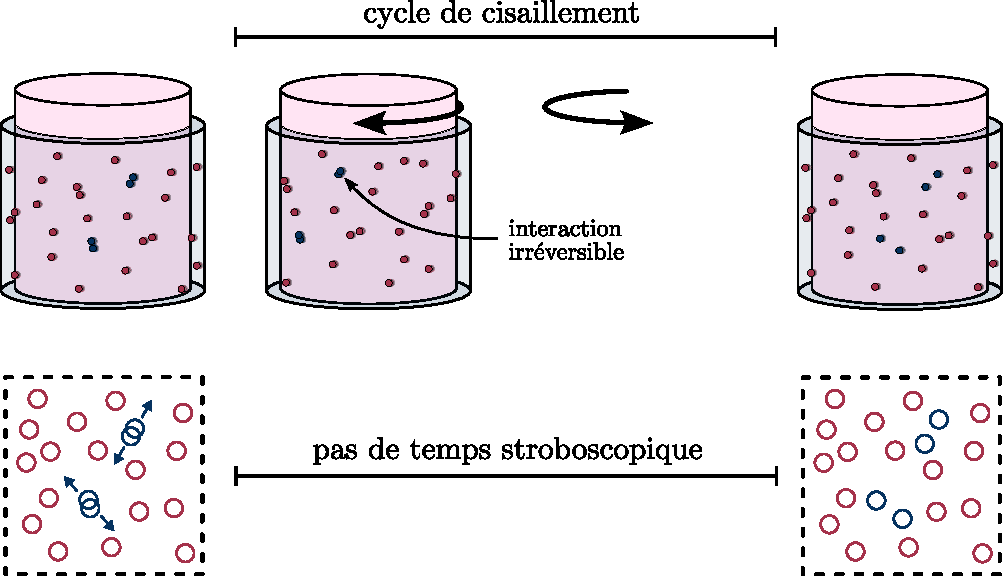
\includegraphics[width=0.85\textwidth]{Chapitre3/Figures/Method/equivROMSusp.pdf}
	\caption{Équivalence entre la vision dynamique et la vision stroboscopique dans les expériences de suspensions cisaillées cycliquement.}
	\label{fig:equivROMSusp}
\end{figure}

\subparagraph{}Toutefois, nous avons vu dans le \autoref{chapter:introduction} que la transition de réversibilité était une transition de phase absorbante avec comme paramètre de contrôle l'amplitude de cisaillement $\gamma_0$ et comme paramètre d'ordre le coefficient de diffusion stroboscopique $D_0$. Il n'est donc pas évident de transposer ces observables au ROM, pour lequel le paramètre de contrôle est la densité de particules $\phi$  et le paramètre d'ordre l'activité $A$. En effet, dans le modèle stroboscopique, la notion de cisaillement est totalement perdue. Pourtant, il est possible de faire un parallèle entre ces deux approches. En fait, dans les expériences et simulations de la transition de réversibilité, l'amplitude de cisaillement critique $\gamma_{0,c}$ est fonction de la densité de particules $\phi$ dans le système. Par exemple dans les expériences de Pine et. al \cite{pine_chaos_2005} et les simulations de Ge et al. \cite{ge_rheology_2022}, il a été observé que $\gamma_{0,c}\sim \phi^{-2}$ comme le montrent les résultats présentés sur la \autoref{fig:phivsgamma}.

\begin{figure}[h]
	\centering
	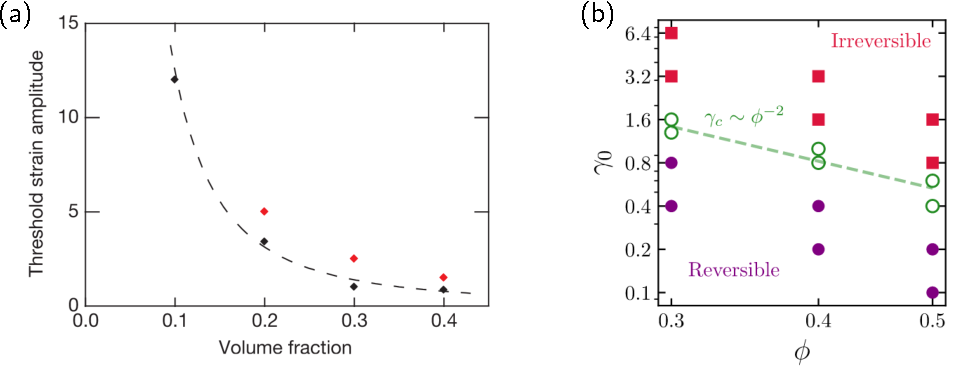
\includegraphics[width=0.9\textwidth]{Chapitre3/Figures/Method/phivsgamma.pdf}
	\caption{Diagrammes de phase des transitions de réversibilité dans les expériences de Pine et al. \cite{pine_chaos_2005} (a) et les simulations de Ge et al. \cite{ge_rheology_2022} (b) montrant l'évolution de l'amplitude de cisaillement critique $\gamma_{0,c}$ avec la densité de particules. Les lignes pointillées représentent la ligne de transition.}
	\label{fig:phivsgamma}
\end{figure}

\noindent Il est donc possible en pratique de passer de l'état absorbant à l'état diffusif en gardant l'amplitude de cisaillement $\gamma_0$ constante et en variant la densité de particules jusqu'à ce que celle-ci définisse $\gamma_{0,c}(\phi) = \gamma_0$. En d'autres termes, la densité de particules représente une autre variable que $\gamma_0$ permettant de traverser la ligne de transition, représentée sur la \autoref{fig:phivsgamma}. Ainsi, elle constitue aussi un paramètre de contrôle de cette transition expérimentale, ce qui permet donc de faire un lien direct avec la modélisation offerte par le ROM. De la même façon, le coefficient de diffusion stroboscopique du système réel est directement relié au nombre de particules interagissant irréversiblement. Ainsi, un paramètre d'ordre équivalent est bien l'activité dans le ROM. En d'autres termes, sous ce prisme, une particule active dans le ROM est une particule interagissant irréversiblement dans la vision dynamique. Par la correspondance $\gamma_0 \rightarrow \phi$ et $D_0\rightarrow A$, le ROM est donc, de par sa simplicité, le modèle numérique idéal pour simuler la transition de réversibilité dans les suspensions cisaillées cycliquement.

\subparagraph{}Suivant ces lignes, comme nous l'avons évoqué au \autoref{chapter:introduction}, Menon et Ramaswamy \cite{menon_universality_2009} ont utilisé cette équivalence pour justifier l'appartenance de cette transition à la classe CDP. Toutefois cette approche omet la présence attendue d'interactions hydrodynamiques entre les particules. Notre objectif est alors de comprendre comment ces interactions à longue portée peuvent affecter la criticalité du système. Or, si le ROM est un modèle efficace pour sonder la transition dans le cas d'interactions à courte portée, il ne permet pas en l'état de modéliser les interactions médiées par le fluide suspendant.

\subsection{Modélisation des interactions médiées}

\subparagraph{}Afin de conserver l'efficacité du modèle stroboscopique tout en y ajoutant la présence d'interactions médiées à longue portée, ces dernières doivent pouvoir être modélisées de manière simple et efficace. Le premier objectif de cette étude est donc de déterminer la modélisation adaptée.

\subparagraph{}En pratique, au cours d'un cycle de cisaillement, chaque particule suspendue dans le fluide interagit avec les autres particules via des interactions hydrodynamiques, dont la forme a été explicitée à la \autoref{sec:ref_interac_visc} et dans l'\annexeref{sec:Annexe_Interactions_Hydro}. Celle-ci suppose un écoulement à bas Reynolds régi par les équations de Stokes et des particules ponctuelles sans inertie. Notamment, un évènement irréversible que l'on associe instantanément à un dipôle de force en $\mathbf{r}^\prime$ sur le fluide induit une vitesse de déplacement $\mathbf{v}^p(\mathbf{r})$ pour une particule située en $\mathbf{r}$ selon\footnote{Nous utilisons ici la convention d'Einstein pour la sommation sur les indices répétés.} :

\begin{equation}
	v^p_i(\mathbf{r}) = \mathcal{G}_{ijk}(\mathbf{r}-\mathbf{r}^\prime)p_{jk}
\end{equation}

\noindent avec $\mathcal{G}_{ijk}(\mathbf{r}-\mathbf{r}^\prime)$ le propagateur hydrodynamique dipolaire, décroissant comme $1/|\mathbf{r}-\mathbf{r}^\prime|^\alpha$ à grande échelle, avec $\alpha$ dépendant de la géométrie considérée. $p_{jk} = F_j a_k$ représente le dipôle de force associé aux deux particules interagissant irréversiblement, appliquant respectivement instantanément une force $\mathbf{F}\delta(\mathbf{r}+\frac{\mathbf{a}}{2})$ et une force $-\mathbf{F}\delta(\mathbf{r}-\frac{\mathbf{a}}{2})$ sur le fluide (voir \annexeref{sec:Annexe_Interactions_Hydro}).

\subparagraph{}En réalité, au cours de la transition réelle, les déplacements irréversibles des particules et donc les forces qu'elles exercent varient au cours d'un cycle. L'effet intégré dans le temps d'un évènement irréversible prend donc une forme complexe, non-instantanée. Afin de modéliser simplement l'influence d'un tel évènement dans son intégralité, nous le considérons donc simplement dans l'approche stroboscopique. Nous considérons alors que chaque couple de particules actives situé autour de $\mathbf{r}^\prime$ génère un dipôle intégré de force $\tilde{p}_{jk}(\mathbf{r}^\prime)$, qui induit un déplacement $\boldsymbol\delta^p(\mathbf{r})$ sur une particule située en $\mathbf{r}$ selon :

\begin{equation}
	\delta^p_i(\mathbf{r}) = \mathcal{G}_{ijk}(\mathbf{r}-\mathbf{r}^\prime)\tilde{p}_{jk}(\mathbf{r}^\prime)
\end{equation}

\noindent avec le même propagateur hydrodynamique que celui associé à l'évènement instantané.

\subparagraph{}Cette modélisation implique une approche tensorielle de l'influence des particules actives sur les particules passives (par opposition à actives) dans le modèle stroboscopique : le déplacement d'une particule passive induit par un couple de particules actives dépend de la direction de déplacement de ces dernières. En s'appuyant sur le fait que, dans la phase active, dans la limite thermodynamique, chaque particule passive reçoit des interactions médiées de la part d'un grand nombre particules actives, on a en notant $\{ \mathbf{r}^\prime \}$ l'ensemble des positions des couples de particules actives :

\begin{equation}
	\delta^p_i(\mathbf{r}) = \sum_{\mathbf{r}^\prime}\mathcal{G}_{ijk}(\mathbf{r}-\mathbf{r}^\prime)p_{jk}(\mathbf{r}^\prime)
\end{equation}

\noindent par linéarité des équations de Stokes. De ce fait, nous pouvons aborder cette interaction d'un point de vue statistique. En considérant les dipôles actifs comme aléatoires, on a $\langle \delta^p_i(\mathbf{r}) \rangle = 0$ avec $\langle \cdot \rangle$ représentant une moyenne sur les dipôles induits par les particules actives. De plus, en considérant les différents dipôles actifs décorrélés entre eux, de force typique $F$ et de distance de séparation typique $a$, on a :

\begin{equation}
\begin{aligned}
	\langle\boldsymbol\delta^p(\mathbf{r})^2\rangle &= \sum_{\mathbf{r}^\prime}\sum_{\mathbf{r}^{\prime\prime}}\mathcal{G}_{ijk}(\mathbf{r}-\mathbf{r}^\prime)\mathcal{G}_{ilm}(\mathbf{r}-\mathbf{r}^{\prime\prime})\langle p_{jk}(\mathbf{r}^\prime)p_{lm}(\mathbf{r}^{\prime\prime})\rangle \\
	&= \sum_{\mathbf{r}^\prime}\sum_{\mathbf{r}^{\prime\prime}}\mathcal{G}_{i\alpha}(\mathbf{r}-\mathbf{r}^\prime)\mathcal{G}_{i\beta}(\mathbf{r}-\mathbf{r}^{\prime\prime})a^2F^2\delta_{\mathbf{r}^\prime\mathbf{r}^{\prime\prime}}\delta_{jl}\delta_{km}\\
	&= a^2 F^2\sum_{\mathbf{r}^\prime}\mathcal{G}_{ijk}(\mathbf{r}-\mathbf{r}^\prime)\mathcal{G}_{ilm}(\mathbf{r}-\mathbf{r}^{\prime})\delta_{jl}\delta_{km}\\
	&= a^2 F^2 \sum_{\mathbf{r}^\prime}\mathcal{G}_{ijk}(\mathbf{r}-\mathbf{r}^\prime)\mathcal{G}_{ijk}(\mathbf{r}-\mathbf{r}^{\prime})
\end{aligned}
\end{equation}

\noindent les sommes sur les indices de coordonnées $i$, $j$ et $k$ étant implicites. Nous considérerons donc simplement dans notre modélisation statistique :

\begin{equation}
	\langle \boldsymbol\delta^p(\mathbf{r})^2 \rangle \sim \sum_{\mathbf{r}^\prime} \mathcal{G}^2(\mathbf{r}-\mathbf{r}^\prime)
	\label{eq:convol_model}
\end{equation}

\noindent avec $\mathcal{G}^2$ un propagateur scalaire effectif de l'interaction, que nous choisissons isotrope et décroissant comme $1/r^{\alpha}$ de la même manière que le propagateur hydrodynamique tensoriel associé.

\subparagraph{}En pratique, Le propagateur scalaire effectif retenu pour la modélisation est de la forme spécifique suivante :

\begin{equation}
	\mathcal{G}^2(\mathbf{r}-\mathbf{r}^\prime) = \frac{c}{\left(1+\left(\frac{|\mathbf{r}-\mathbf{r}^\prime|}{D_p}\right)^2\right)^\alpha}, \quad c > 0
\end{equation}

\noindent avec $D_p$ le diamètre des particules et $c$ un paramètre représentant la borne supérieure de l'interaction. Cette formulation modélise alors bien une interaction entre particules actives et particules passives qui décroît comme $1/r^\alpha$ en champ lointain. La régularisation en $|\mathbf{r}-\mathbf{r}^\prime|=0$ permet par ailleurs de considérer sans difficulté des interactions pour lesquelles on a $2\alpha > D$, sans quoi cette forme ne serait plus intégrable. Pour $2\alpha < D$, la non-intégrabilité du propagateur en $|\mathbf{r}|\rightarrow\infty$ et sa prise en compte dans le modèle sera discutée à la \autoref{sec:noninteg}.

\subparagraph{}In fine, sous ce point de vue statistique, nous considérons que chaque particule passive effectue à chaque pas de temps stroboscopique un déplacement aléatoire gaussien de moyenne nulle et de variance donnée par l'\autoref{eq:convol_model}. Ces simplifications permettent alors de rendre la modélisation des interactions scalaire, ce qui permet d'alléger fortement l'implémentation numérique que nous détaillons dans la partie suivante.

\subsection{Implémentation numérique}

\label{sec:ImplNumTBLRR}

\subparagraph{}Pour l'implémentation numérique de ce modèle, nous reprenons les éléments de base du ROM, détaillés au \autoref{chapter:TransportLP}. Les interactions médiées représentent alors simplement une composante additionnelle à ce modèle, à implémenter à chaque pas de temps. 

\subsubsection{Calcul de l'influence des particules actives}

\subparagraph{}Afin de simplifier le calcul numérique de la somme de l'\autoref{eq:convol_model}, nous choisissons de considérer une version gros grains de l'activité dans le système. Pour ce faire, nous définissons un champ d'activité discret $A(\mathbf{r}_i)$, défini sur le réseau utilisé pour la méthode cell-list, introduite à la \autoref{sec:DetImpl}. Chaque case du réseau est alors définie autour d'une position $\mathbf{r}_i = na\hat{\mathbf{e}}_x + ma \hat{\mathbf{e}}_y$ avec $(n,m) \in \mathbb{Z}^2$ et $a$ le pas du réseau que l'on prend de nouveau égal à $D_p=1$. \`A chaque pas de temps, après identification des particules actives, nous calculons ce champ d'activité sur la case du réseau centrée autour de $\mathbf{r}_i$ comme le nombre de particules actives dans cette case (voir \autoref{fig:modelsusp}). $A(\mathbf{r}_i)$ représente alors en quelque sorte une quantité d'activité locale.

\begin{figure}[h]
	\centering
	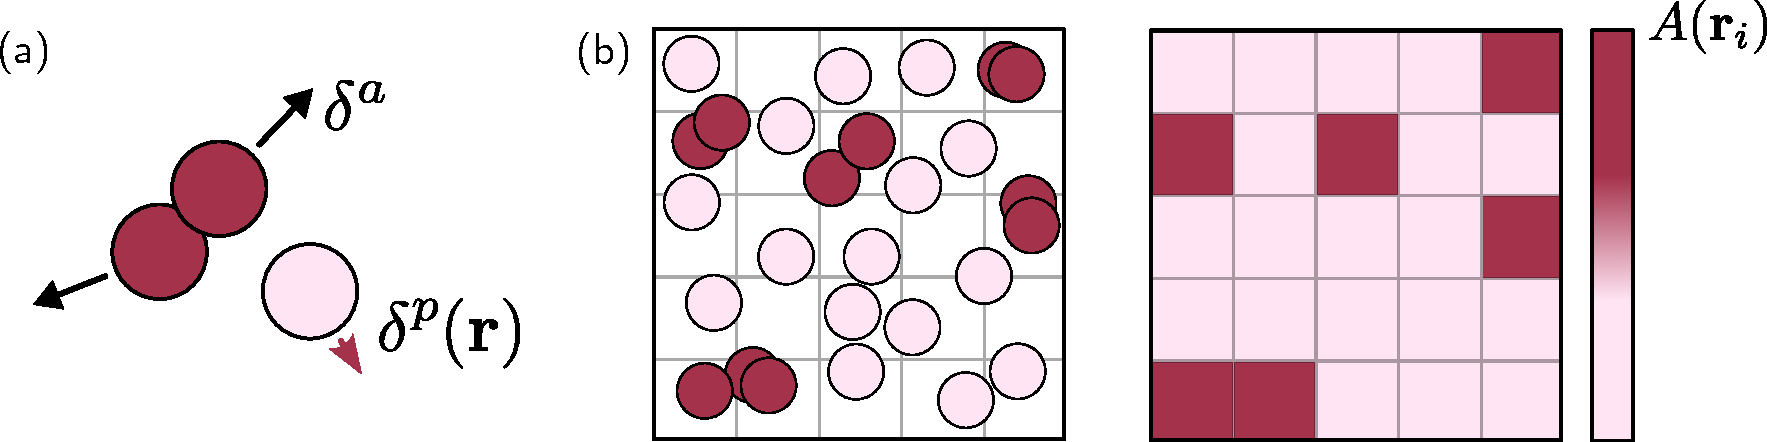
\includegraphics[width=0.9\textwidth]{Chapitre3/Figures/Method/Model.pdf}
	\caption{Implémentation numérique du modèle $\alpha$-ROM. (a) Les particules actives (rouges) sont soumises à des déplacements aléatoire $\boldsymbol\delta^a$ indépendants de leur position. Les particules passives sont soumises à des déplacements aléatoires $\boldsymbol\delta^p$ dont l'amplitude typique dépend de leur distance à l'activité. (b) Méthode de détermination du champ d'activité discret $A(\mathbf{r}_i)$.}
	\label{fig:modelsusp}
\end{figure}

\subparagraph{}Pour déterminer la variance du déplacement des particules passives à chaque pas de temps, il suffit donc de calculer la convolution discrète suivante :

\begin{equation}
	\langle \boldsymbol\delta^p(\mathbf{r}_i)^2\rangle = \sum_{j} G^2(\mathbf{r}_i-\mathbf{r}_j) A(\mathbf{r}_j)
	\label{eq:kick_discret}
\end{equation}

\noindent avec $G^2$ la version discrétisée du propagateur $\mathcal{G}^2$. Cette convolution étant définie sur un réseau régulier, il est possible de la calculer efficacement en passant par l'espace de Fourier. En pratique, nous la calculons donc dans l'espace réciproque où elle devient le simple produit $\hat{G^2}(\mathbf{q}_i)\hat{A}(\mathbf{q}_i)$, avec $\mathbf{q}_i = (\frac{2\pi}{L}n, \frac{2\pi}{L}m)$ et $L$ la taille du système. La notation $\hat{\cdot}$ définit alors ici la transformée de Fourier discrète sur ce réseau. Pour ce faire, nous définissons directement le propagateur hydrodynamique dans l'espace de Fourier. Dans le cas continu, le calcul relégué dans l'\annexeref{sec:TFinverse_susp} donne en deux dimensions :

\begin{equation}
	\hat{\mathcal{G}^2}(\mathbf{q})=\frac{2\pi c}{\Gamma\left(\alpha\right)} \left( \frac{q}{2} \right)^{\alpha-1}K_{\alpha-1}(q)
	\label{eq:propcontinu2D}
\end{equation}

\noindent avec $\Gamma$ la fonction Gamma d'Euler et $K_{\alpha -1}$ la fonction de Bessel modifiée de seconde espèce d'ordre $\alpha - 1$ \cite{abramowitz_handbook_1965}. On peut alors estimer la valeur de ce propagateur continu en $\mathbf{q}=0$ pour un milieu de taille finie en calculant sa valeur moyenne dans l'espace réel :

\begin{equation}
	\hat{\mathcal{G}^2}(0) = \frac{\pi c}{\alpha -1}\left( 1- \left( 1+L^2 \right)^{1-\alpha} \right) \xrightarrow[L\rightarrow\infty]{\alpha > 1} \frac{\pi c}{\alpha - 1}
	\label{eq:zerovalue}
\end{equation}

\noindent Nous choisissons donc de définir le propagateur discret $\hat{G^2}$ dans l'espace réciproque via l'expression :

\begin{equation}
	\hat{G^2}(\mathbf{q}_i) = \hat{\mathcal{G}^2}(q), \quad q = \sqrt{\left( 2-2\cos \left( \frac{2\pi}{L}n \right) \right) + \left( 2-2\cos \left( \frac{2\pi}{L}m \right) \right)}
\end{equation}

\noindent la conversion du nombre d'onde sous sa forme discrète étant essentielle pour définir proprement le propagateur dans l'espace réciproque discret \cite{ferrero_criticality_2019, rossi_finite-disorder_2022}, comme nous l'expliquons dans l'\annexeref{sec:impl_disc_propag}.

\subparagraph{}Finalement, la valeur réelle de la convolution est obtenue en opérant une transformée de Fourier inverse discrète sur le produit. La forme alors obtenue par cette procédure pour $\alpha \in \{ 3, 2, 1.5 \}$ est présentée à la \autoref{fig:PropagTBLRR}-(a). Cette méthode de calcul de la convolution étant parallélisable, elle nous permet de conserver l'architecture GPU utilisée pour les simulations des modèles LR-ROM et LR-Manna. De plus, la méthode pseudo-spectrale permet de prendre en compte les conditions aux limites périodiques du système naturellement. Enfin, afin d'optimiser notre utilisation des fonctions de Fast Fourier Transform \cite{cooley_algorithm_1965}, nous privilégions les tailles de système de la forme $L = 2^p$ avec $p \in \mathbb{N}$.

\subparagraph{}De cette manière, en plus des particules actives, les particules passives sont soumises à un déplacement dont la variance est donnée par l'\autoref{eq:kick_discret} à chaque pas de temps. Ce modèle représente alors une généralisation du modèle étudié par Mari et al. \cite{mari_absorbing_2022}. En effet, celui-ci correspond en fait exactement au cas $\alpha = 0$ (et donc des interactions médiées indépendantes de la distance) qui correspond bien à une limite champ moyen de la prise en compte des interactions hydrodynamiques.

\subparagraph{}L'ajout de ce nouveau mécanisme de diffusion des particules passives conserve la présence d'une transition de phase absorbante analogue à celle du ROM et dont les propriétés critiques varient avec la portée de l'interaction $\alpha$. Nous appelons alors ce nouveau modèle $\alpha$-ROM, et, par analogie, celui de Mari et al. 0-ROM. 

\subsubsection{Non-intégrabilité du propagateur à longue portée}

\label{sec:noninteg}

\subparagraph{}Si la régularisation du propagateur en $r=0$ permet de le rendre intégrable pour $2\alpha > D$, pour $2\alpha<D$ c'est la limite $r\rightarrow\infty$ qui pose problème. En effet, dans ce cas, la valeur moyenne du propagateur diverge comme $L^{2-2\alpha}$ pour $L$ grand. Si cette divergence n'est pas un problème en soi pour l'étude d'un système de taille finie, elle en représente un pour la comparaison des comportements critiques à différentes tailles. En effet, cette dépendance du propagateur en taille rend la densité critique $\phi_c$ elle aussi fortement dépendante de $L$ (voir \autoref{fig:PropagTBLRR}-(b)). De ce fait, il n'est alors plus possible d'utiliser différentes tailles du système pour sonder le comportement critique à une portée $\alpha$ donnée, comme cela a été fait à la \autoref{sec:expcritjumps} dans le cas des sauts à longue portée.

\subparagraph{}Afin de remédier à ce problème, nous choisissons de normaliser les propagateurs pour $2\alpha<D$ par un facteur $L^{2-2\alpha}$, rendant de ce fait la valeur moyenne du propagateur indépendante de la taille du système. Par cette procédure, nous retrouvons alors pour $\alpha = 0.5$ une densité critique indépendante de la taille du système à grande taille (voir \autoref{fig:PropagTBLRR}-(c)). Toutefois pour $\alpha = 1$, pour lequel la divergence de la valeur moyenne du propagateur évolue de manière logarithmique avec la taille, cette procédure de normalisation par un facteur $\ln (L)$ n'est pas concluante. En effet, dans ce cas, $\phi_c$ montre une forte dépendance avec la taille du système même après normalisation. Ceci peut être expliqué par le fait qu'une telle divergence logarithmique n'est valable qu'à des tailles de systèmes excessivement grandes. Ce cas restant néanmoins d'intérêt, nous conservons son étude mais nous nous limitons pour cela à une taille de système fixée.

\begin{figure}[h]
	\centering
	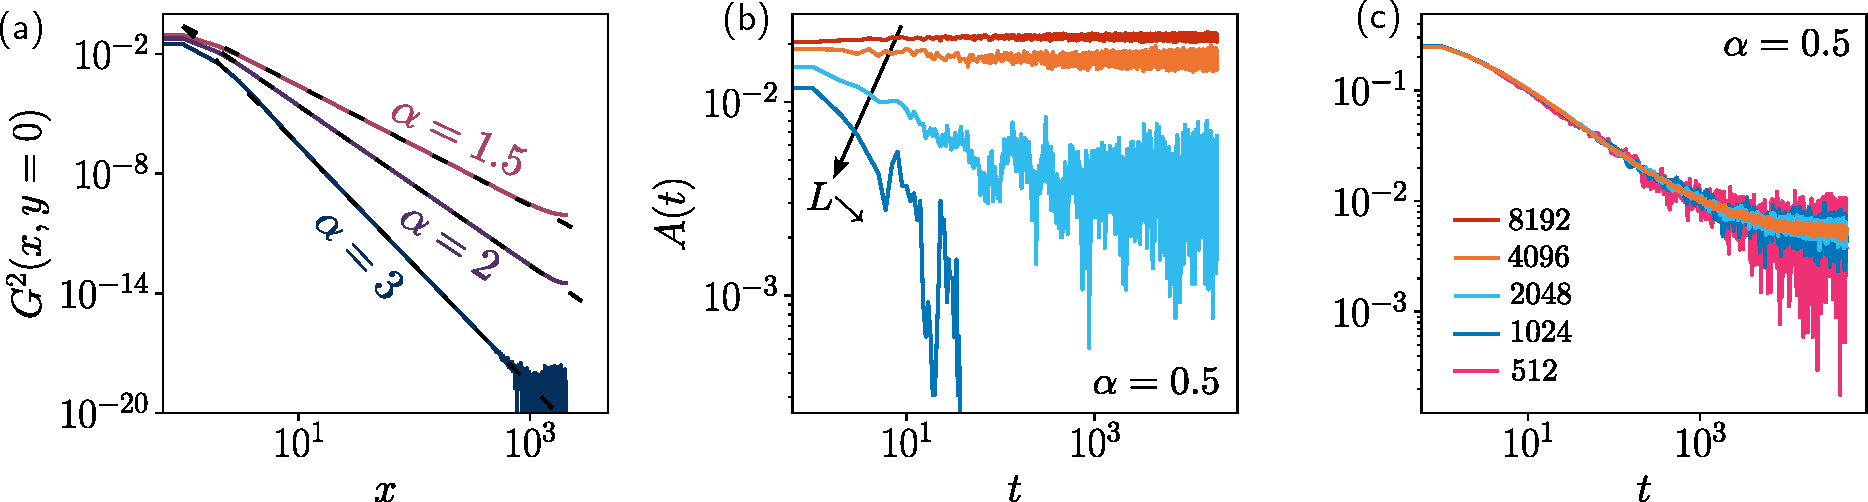
\includegraphics[width=\textwidth]{Chapitre3/Figures/Method/PropagTBLRR2D.pdf}
	\caption{Propagateurs d'interaction dans le modèle $\alpha$-ROM. (a) Évolution du propagateur effectif dans l'espace discret réel pour $\alpha \in \{ 3, 2, 1.5 \}$. Les pointillés noirs représentent les lois de puissance $1/r^{2\alpha}$. (b) Évolution de l'activité vers l'état stationnaire à $\phi = 0.00486859$ pour différentes tailles de système avec $\alpha = 0.5$ dans le cas d'un propagateur non normalisé. La distinction des courbes montre un point critique nettement différent pour chaque taille. (c) Idem à $\phi=0.101117$ avec le propagateur normalisé.}
	\label{fig:PropagTBLRR}
\end{figure}

\subsubsection{Extension aux dimensions supérieures}

\subparagraph{}Notre travail se focalise sur une étude de la transition en deux dimensions. Toutefois, certains cas physiques de cette transition ont lieu dans un espace de trois dimensions \cite{pine_chaos_2005}. De plus, d'un point de vue purement théorique, il peut être intéressant de comprendre comment cette transition évolue avec le nombre de dimensions du système. Pour ces raisons, nous généralisons cette méthode de simulation numérique à $n$ dimensions.

\subparagraph{}La complexité de cette implémentation réside alors essentiellement dans l'intégration des conditions aux limites périodiques. Dans le cas du calcul des interactions à longue portée, celles-ci sont directement prises en compte par la méthode pseudo-spectrale. Pour le calcul des interactions de contact cependant, la périodicité nécessite plus d'attention, mais reste généralisable grâce à un peu d'algèbre. 

%L'algorithme obtenu a alors été testé à courte portée (dans le cas du ROM donc) pour $D=3$ et $D=4$. Son bon fonctionnement a alors été attesté par la mesure des exposants critiques $\beta$ dans ces deux dimensions, qui correspondent alors bien à ceux attendus pour la classe CDP.

\subparagraph{}Afin de mesurer de manière annexe le comportement critique du $\alpha$-ROM en 3D, nous implémentons les interactions médiées de la même façon qu'en 2D. Seulement, cette fois, la forme spectrale continue du propagateur est\footnote{Le calcul est relégué dans l'\annexeref{sec:TFinverse_susp}} :

%\begin{equation}
%	\hat{\mathcal{G}}(\mathbf{q}) = \frac{c\pi^\frac{3}{2}2^{\frac{5}{2}-\alpha}}{\Gamma (\alpha)}q^{\alpha-\frac{3}{2}}K_{\alpha-\frac{3}{2}}(q),\quad \hat{\mathcal{G}}(0) \xrightarrow{\alpha > \frac{3}{2}} c \pi^{\frac{3}{2}}\frac{\Gamma\left(\alpha-\frac{3}{2}\right)}{\Gamma (\alpha)}
%\end{equation}

\begin{equation}
	\hat{\mathcal{G}^2}(\mathbf{q}) = \frac{c\pi^\frac{3}{2}2^{\frac{5}{2}-\alpha}}{\Gamma (\alpha)}q^{\alpha-\frac{3}{2}}K_{\alpha-\frac{3}{2}}(q)
\end{equation}

\noindent Pour $\alpha < \frac{3}{2}$, nous opérons la même procédure de normalisation que pour le cas 2D mais seulement cette fois par le facteur $L^{3-2\alpha}$.

\subsection*{Bilan}

\subparagraph{}Finalement le modèle ainsi implémenté du $\alpha$-ROM nous permet d'étudier efficacement les transitions de phase absorbantes associées à chaque portée de l'interaction médiée $\alpha$ en deux et trois dimensions. Grâce à cet outil, il est alors possible de comprendre comment l'on passe du cas limite de courte portée du ROM ($\alpha\rightarrow\infty$), représenté par la classe CDP, au cas limite $\alpha \rightarrow 0$, représenté par une transition convexe et des fluctuations critiques évanescentes \cite{mari_absorbing_2022}, totalement hors du cadre théorique LR-CDP.

\section{Comportement critique}

\subparagraph{}Afin de déterminer l'évolution de la criticalité du système avec la portée d'interaction $\alpha$, nous commençons par déterminer le comportement critique statique des modèles $\alpha$-ROM. Pour ce faire, nous caractérisons d'abord en 2D la gamme de portées suivante : $\alpha \in \{ 0.5, 1, 1.25, 1.5, 1.75, 2, 3 \}$ et nous mesurons les exposants critiques $\beta$ et $\gamma^\prime$. 

\subsection{Détermination du point critique}

\subparagraph{}Nous commençons tout d'abord par déterminer les densités critiques $\phi_c$ associées à chaque transition. En utilisant des tailles de systèmes allant de $L=2048$ à $L=8192$, nous mesurons l'activité moyenne $\langle A \rangle$ dans l'état stationnaire pour différentes densités $\phi$ et ce pour chaque portée $\alpha$. Pour le cas problématique $\alpha=1$ évoqué précédemment, le comportement critique est évalué pour la plus grande taille $L=8192$. En estimant grossièrement la densité critique associée à chaque portée il est alors possible de tracer les courbes d'évolution du paramètre d'ordre, représentées à la \autoref{fig:qualideter}-(a).

\begin{figure}[h]
	\centering	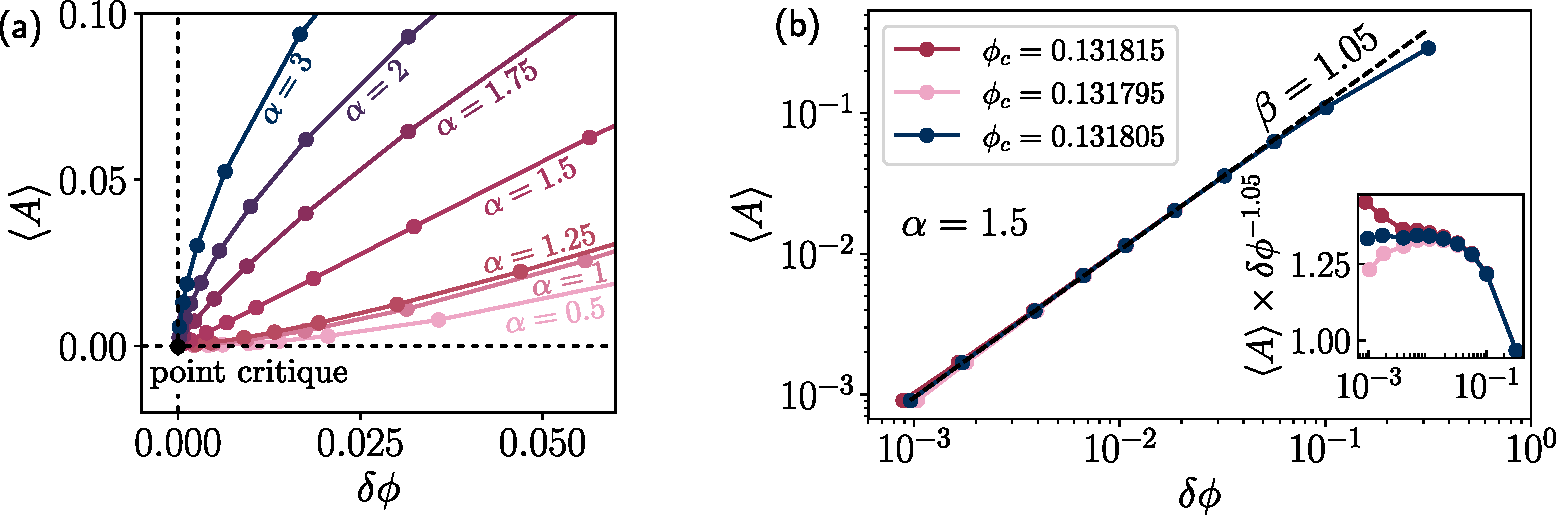
\includegraphics[width=\textwidth]{Chapitre3/Figures/BetaGamma/EvolMeanDeter.pdf}
	\caption{(a) Évolution de l'activité moyenne dans l'état stationnaire avec la distance au point critique pour différentes portées $\alpha$ des interactions médiées en 2D. (b) Exemple de détermination d'une densité critique $\phi_c$ dans le cas $\alpha = 1.5$ en 2D. Le choix $\phi_c = 0.131805$ est significativement meilleur que $\phi_c = 0.131815$ et $\phi_c = 0.131795$. En encart, la représentation compensée permet d'exacerber ces différences.}
	\label{fig:qualideter}
\end{figure}

\subparagraph{}Nous remarquons que cette évolution passe effectivement d'une forme concave à grand $\alpha$, à une forme convexe à petit $\alpha$. Ce comportement qualitatif est donc en accord avec les limites de courte portée ($\beta  \approx 0.64$ \cite{lubeck_universal_2004}) et de portée infinie ($\beta\approx 1.85$ \cite{mari_absorbing_2022}). Ainsi, comme dans le cas des sauts à longue portée, la criticalité semble évoluer continûment avec la portée de l'interaction.

\subparagraph{}Afin d'évaluer plus quantitativement cette évolution, il nous faut mesurer précisément l'exposant $\beta$ associé. Nous reprenons alors la méthode présentée à la \autoref{sec:methodchap2}. Un exemple de détermination dans le cas du $\alpha$-ROM pour $\alpha = 1.5$ est représenté à la \autoref{fig:qualideter}-(b). Ces déterminations sont alors bien plus compliquées que dans le cas des sauts à longue portée et ce pour deux raisons principales. La première est que le régime stationnaire est bien plus long à atteindre en présence de la diffusion des particules passives. Notamment, la décroissance initiale de l'activité et la transition entre régime transitoire et régime stationnaire associés sont bien moins abrupts. Ainsi, pour une courbe de convexité équivalente (i.e. $\beta$ équivalent), les simulations nécessitent plus de dix fois plus de pas de temps avant équilibration\footnote{De plus, les pas de temps du $\alpha$-ROM sont bien plus coûteux en termes de ressources numériques puisqu'ils font intervenir des calculs de FFT.}. La seconde vient du fait que les transitions convexes sont plus difficiles à caractériser. En effet, pour une distance au point critique équivalente, celles-ci impliquent des valeurs d'activités bien plus faibles (puisque $\langle A \rangle \sim \delta\phi^\beta$). Cela requiert alors des tailles de systèmes plus grandes et donc des simulations plus longues. Au final, l'équilibration de certains points aura nécessité plus de 800 heures de simulation continue sur des cartes graphiques de nouvelle génération\footnote{Les simulations présentées dans cet ouvrage ont été principalement réalisées sur des clusters de calcul GPU permettant un accès à des cartes graphiques NVIDIA V100 et A100.}. En général, la caractérisation des transitions convexes amènera donc plus d'incertitudes.

\subsection{Évolution des exposants critiques}

\subsubsection{Exposants statiques}

\label{sec:TBLRRStat}

\subparagraph{}Les densités critiques déterminées permettent de représenter les courbes $\langle A \rangle = f(\delta\phi)$ en échelle logarithmique pour chaque $\alpha$ sur la \autoref{fig:evolmeanvar}-(a). Les exposants $\beta$ estimés par cette méthode sont reportés dans le \autoref{tab:expocrit_alphaROM}-(a) et leur évolution est résumée sur la \autoref{fig:expcritTBLRR}-(a).

\begin{figure}[h]
	\centering
	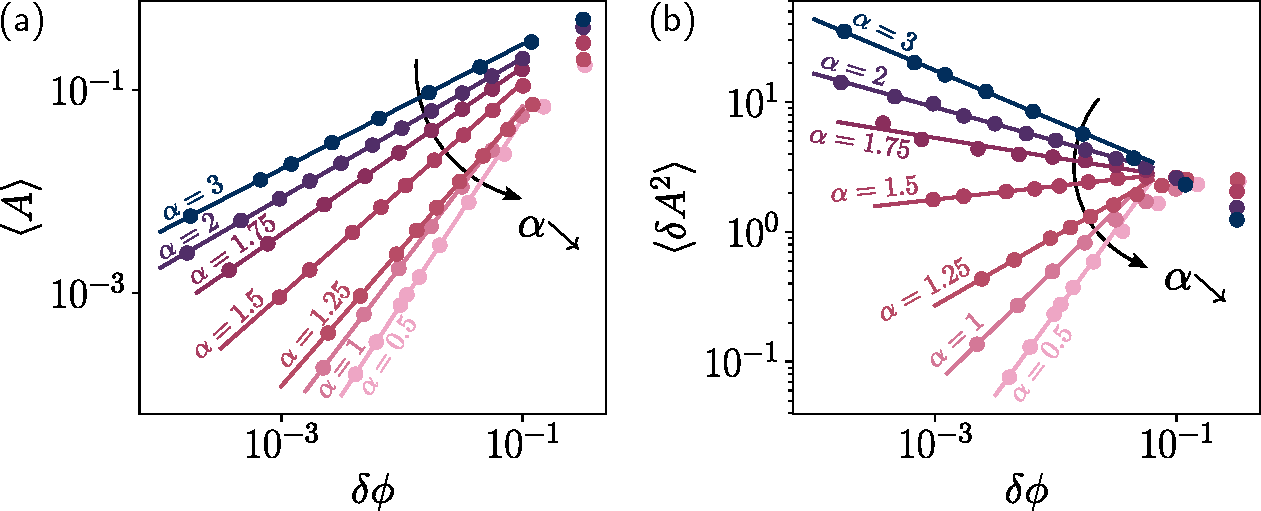
\includegraphics[width=0.9\textwidth]{Chapitre3/Figures/BetaGamma/EvolMeanVar_edited.pdf}
	\caption{(a) Évolution de la valeur moyenne de l'activité dans l'état stationnaire $\langle A \rangle$ en fonction de la distance au point critique $\delta\phi$ à différentes portées dans le $\alpha$-ROM en 2D. (b) Idem pour les fluctuations $\langle \delta A^2\rangle = L^D\times(\langle A ^2 \rangle - \langle A \rangle^2)$.}
	\label{fig:evolmeanvar}
\end{figure}

\subparagraph{}Pour déterminer l'exposant $\gamma^\prime$, comme dans le \autoref{chapter:TransportLP}, nous mesurons $\langle \delta A^2\rangle$ dans l'état stationnaire. La détermination de $\phi_c$ étant déjà effectuée, l'exposant se mesure par un simple ajustement de la courbe en échelle logarithmique. L'évolution des fluctuations en fonction de la portée est alors représentée sur la \autoref{fig:evolmeanvar}-(b). Nous observons un passage de fluctuations divergentes à l'approche du point critique pour les courtes portées à des fluctuations qui s'annulent pour les longues portées. Cette observation est à nouveau en accord avec les comportements limites de courte portée (CDP) et de portée infinie ($0$-ROM). Les valeurs des exposants $\gamma^\prime$ sont reportées dans le \autoref{tab:expocrit_alphaROM}-(a) et leur évolution est résumée sur la \autoref{fig:expcritTBLRR}-(a).

\begin{table}[h]
\centering
\begin{subtable}[t]{0.4\textwidth}
\begin{tabular}{ccccc}
\hline \hline $\alpha$ & $\beta$ & $\gamma^\prime$ & $\delta$ & $\nu_\perp^*$ \\
\hline \text{CDP} \cite{lubeck_universal_2004} & 0.64 & 0.37 & 0.42 & 0.80 \\
3 & 0.62 & 0.39 & 0.41 & 0.82 \\
2 & 0.69 & 0.26 & 0.42 & 0.82 \\
1.75 & 0.82 & 0.15 & 0.45 & 0.90 \\
1.5 & 1.05 & -0.10 & 0.49 & 1.00 \\
1.25 & 1.37 & -0.54 & 0.54 & 1.10 \\
1 & 1.56 & -0.90 & 0.62 & 1.11 \\
0.5 & 1.82 & -1.28 & 0.67 & 1.18 \\
0 \cite{mari_absorbing_2022} & 1.85 & -1.2 & - & 1.3 \\
\hline \hline
\end{tabular}
\caption{}
\end{subtable}
\hspace{0.1\textwidth}
\begin{subtable}[t]{0.4\textwidth}
\begin{tabular}{ccccc}
\hline \hline $\alpha$ & $\beta$ & $\gamma^\prime$ & $\delta$ & $\nu_\perp^*$ \\
\hline \text{CDP} \cite{lubeck_universal_2004} & 0.84 & 0.15 & 0.75 & 0.59 \\
3.5 & 0.84 & 0.16 & 0.74 & 0.61 \\
3 & 0.85 & 0.11 & 0.74 & 0.60 \\
2.5 & 0.95 & -0.03 & 0.74 & 0.62 \\
2 & 1.30 & -0.44 & 0.76 & 0.72 \\
1.75 & 1.49 & -0.82 & 0.75 & 0.72 \\
\hline \hline
\end{tabular}
\caption{}
\end{subtable}
\caption{Exposants critiques déterminés dans les modèles $\alpha$-ROM en 2D (a) et en 3D (b).}
\label{tab:expocrit_alphaROM}
\end{table}

\begin{figure}[h]
	\centering	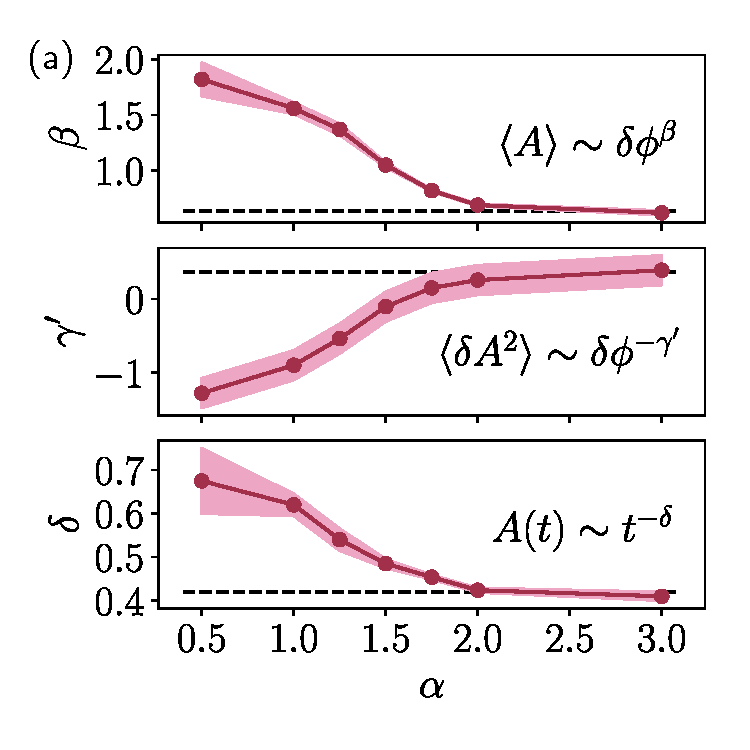
\includegraphics[width=0.48\textwidth]{Chapitre3/Figures/BetaGamma/exp_suspensions.pdf}
	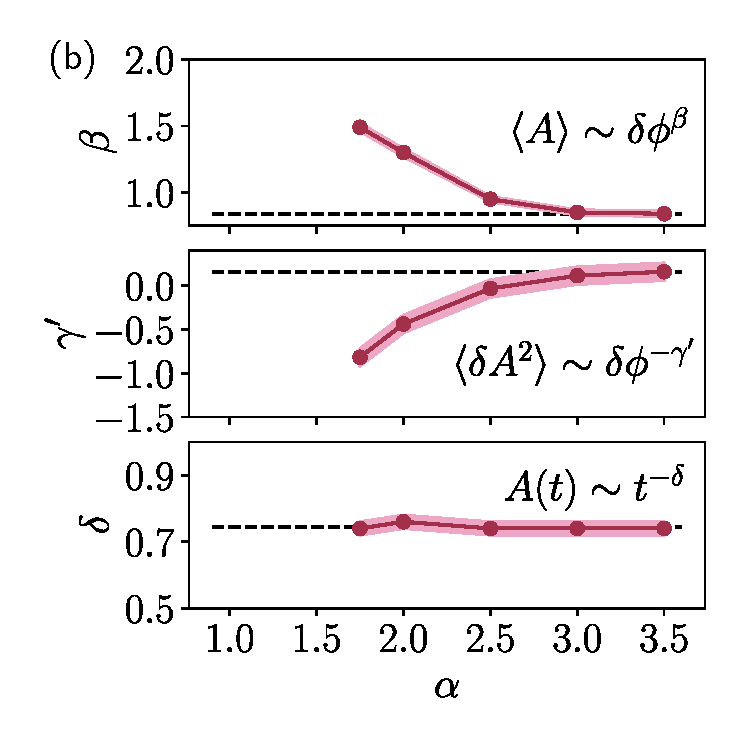
\includegraphics[width=0.48\textwidth]{Chapitre3/Figures/BetaGamma/exp_suspensions3D.pdf}
	\caption{Évolution des exposants critiques $\beta$, $\gamma^\prime$ et $\delta$  avec la portée dans le modèle $\alpha$-ROM en 2D (a) et en 3D (b). Les zones colorées rose représentent les incertitudes de détermination.}
	\label{fig:expcritTBLRR}
\end{figure}

\paragraph{Zones d'évolution}

\subparagraph{}\`A la lumière de la \autoref{fig:expcritTBLRR}-(a), nous observons effectivement une évolution continue des deux exposants avec la portée. Notamment, l'évolution est significative entre $\alpha\approx 2$ et $\alpha \approx 1-0.5$, au-delà de quoi elle semble arriver à saturation des deux côtés\footnote{Pour $\alpha = 0.5$ la saturation se remarque par comparaison avec les valeurs obtenues pour $\alpha = 0$ \cite{mari_absorbing_2022}.}. Par ailleurs les valeurs des exposants aux plus grands $\alpha$ rejoignent celles de la classe CDP : pour $\alpha=3$, l'accord est exact aux incertitudes de détermination près et pour $\alpha=2$ la différence est minime. Cela suggère donc de considérer $\alpha\approx 2$ comme limite de courte portée de la transition. \`A l'opposé du spectre, les exposants déterminés pour $\alpha = 0.5$ rejoignent aussi ceux déterminés dans le cas du $0$-ROM. Cette observation suggère alors $\alpha\approx 0.5$ comme la limite champ moyen de la transition. 

\paragraph{Comportement exotique et point singulier}

\subparagraph{}La spécificité de la limite de portée infinie rend cette variation du comportement critique avec la portée physiquement significative. En effet, si la courbe décrivant l'évolution du paramètre d'ordre reste concave ($\beta < 1$) pour $\alpha \gtrsim 1.5$, celle-ci change de convexité ($\beta >1$) pour $\alpha \lesssim 1.5$. C'est aussi autour de ce même point $\alpha \approx 1.5$ que le comportement des fluctuations critiques s'inverse, passant de divergent à évanescent. Le comportement exotique du 0-ROM est donc retrouvé, de manière qualitative, dans toute la gamme d'évolution $\alpha \lesssim 1.5$. Il est donc envisageable de l'observer dans des systèmes réels présentant des interactions hydrodynamiques spatialisées.

\subparagraph{}Dans le cas du 0-ROM, cette double spécificité $\beta>1$, $\gamma^\prime<0$ peut être rationalisée dans le cadre de la relation d'hyperscaling \cite{lubeck_universal_2004, mari_absorbing_2022} :

\begin{equation}
	2\beta + \gamma^\prime = \nu_\perp D
\end{equation}

\noindent qui se retrouve vérifiée. Celle-ci permet en effet d'expliquer qu'une transition avec une valeur de $\beta$ anormalement grande donne lieu à une valeur de $\gamma^\prime$ anormalement petite. Étant donné que cette relation est aussi vérifiée dans la limite de courte portée CDP, nous pouvons supposer qu'elle l'est en fait dans toute la zone d'évolution présentée par le $\alpha$-ROM. Ainsi, l'annulation des fluctuations critiques s'expliquerait par la convexité de la transition à toute portée $\alpha \lesssim 1.5$.

\subparagraph{}Par ailleurs, si nous allons au bout de notre hypothèse, la relation d'hyperscaling permet de dériver pour chaque $\alpha$ un exposant de corrélation spatiale $\nu_\perp^*$\footnote{Nous utilisons la notation * pour signifier que cette valeur est dérivée d'une relation d'échelle et non mesurée.}. Dans le \autoref{tab:expocrit_alphaROM}-(a), nous répertorions le résultat de cette dérivation. Cet exposant hypothétique $\nu_\perp^*$ semble alors suivre une évolution continue avec la portée $\alpha$ qui lie les deux limites de CDP et du 0-ROM.

\subparagraph{}Le point $\alpha\approx 1.50$ se positionne donc à un changement drastique des propriétés de la transition. Remarquablement, ce point spécifique est décrit les exposants critiques $\beta$ et $\gamma^\prime$ associés au champ moyen de CDP. Une différence majeure est alors que, dans le cas des interactions actives-passives, au contraire du cas des sauts à longue portée étudiés au \autoref{chapter:TransportLP}, ce comportement n'est pas une limite mais il est effectivement dépassé pour des portées plus grandes.

\paragraph{Une limite non triviale}

\subparagraph{}En général, les champs moyens des théories critiques amènent à des valeurs simples des exposants critiques ($\beta_\text{CDP}^\text{CM}=1$ par exemple). Or ici, la limite de portée infinie atteinte en $\alpha=0.5$, tout comme le 0-ROM étudié par Mari et al. \cite{mari_absorbing_2022}, est caractérisée par des exposants non-triviaux. Ces mesures peuvent alors suggérer que cette limite n'est en fait pas un équivalent champ moyen du système. 

\subparagraph{}Cette observation n'est pas si surprenante car certains éléments de la dynamique restent non-triviaux, même à portée infinie. En effet, même lorsque les interactions actives-passives sont à longue portée, les particules actives effectuent des sauts de taille finie et dans un espace de dimension finie. De plus, les particules passives, diffusent elles aussi dans un espace de dimension finie. La dimension de l'espace étant inférieure à la dimension critique supérieure de CDP $D_c = 4$, il est probable que ces mécanismes éloignent le modèle du champ moyen, même si les interactions médiées sont sous leur forme extrémale. Nous pouvons cependant nous attendre à approcher ce champ moyen en augmentant la dimension de l'espace\footnote{Nous reviendrons sur cette idée à la \autoref{sec:interpret}.}.

\subsubsection{Exposant dynamique}

\label{sec:TBLRRdyn}

\subparagraph{}Une autre possibilité pour caractériser la criticalité et son évolution avec la portée est d'étudier la transition d'un point de vue dynamique. Comme dans le cas du transport à longue portée, proche du point critique, le système relaxe vers l'état stationnaire de manière algébrique :

\begin{equation}
	 \langle A \rangle (t) \sim t^{-\delta}
\end{equation}

\noindent $\delta$ définissant un exposant critique universel. Il peut être alors intéressant de comprendre comment celui-ci varie avec $\alpha$ dans le cas du $\alpha$-ROM, et comment cette évolution se compare à l'évolution des exposants $\beta$ et $\gamma^\prime$.

\subparagraph{}Pour aborder cette question, nous reprenons la méthode de redimensionnement utilisée à la \autoref{sec:expdynjump}. Pour chaque $\alpha$, nous déterminons alors l'exposant $\delta$ associé en se basant sur les mesures précédentes de $\beta$ et $\phi_c$. Un exemple de redimensionnement obtenu dans le cas du $\alpha$-ROM est représenté à la \autoref{fig:deltadeter} pour $\alpha = 1.5$. Les valeurs mesurées pour chaque portée sont reportées dans le \autoref{tab:expocrit_alphaROM}-(a) et leur évolution est représentée sur la \autoref{fig:expcritTBLRR}-(a).

\begin{figure}[h]
	\centering
	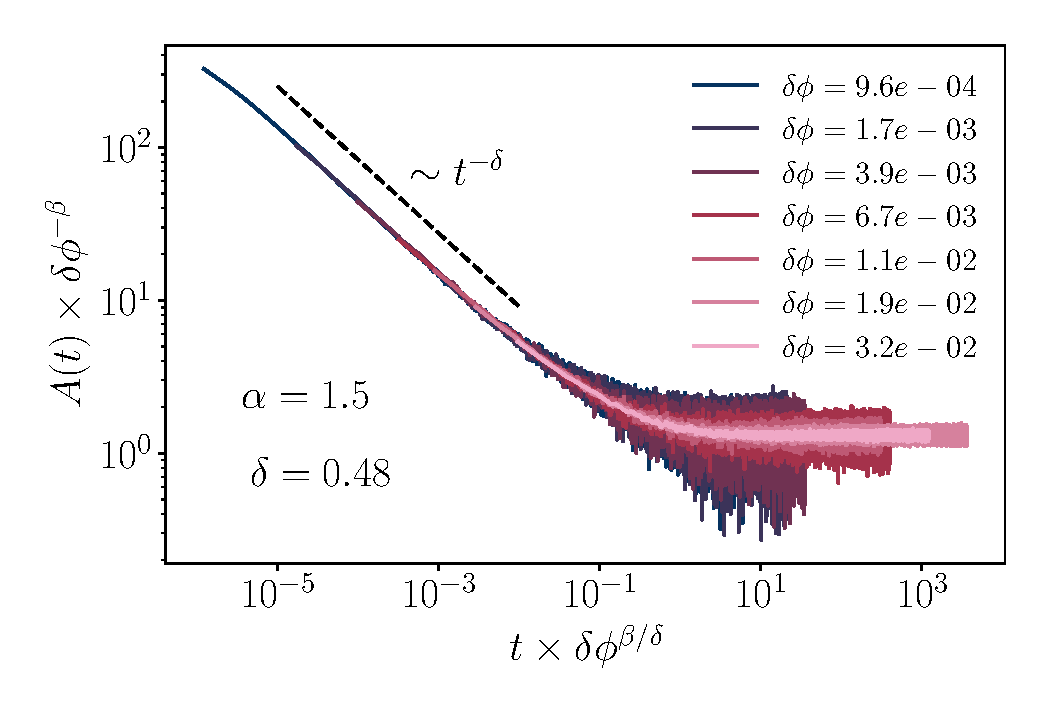
\includegraphics[width=0.7\textwidth]{Chapitre3/Figures/Delta/DeltaDetermination.pdf}
	\caption{Redimensionnement avec la distance au point critique $\delta\phi$ des évolutions de l'activité $A$ avec le temps $t$ dans le cadre du $\alpha$-ROM en 2D pour $\alpha = 1.5$.}
	\label{fig:deltadeter}
\end{figure}

\subparagraph{}Comme pour les exposants $\beta$ et $\gamma^\prime$, l'exposant dynamique $\delta$ évolue de sa valeur CDP pour $\alpha\gtrsim 2$ à une valeur de saturation pour $\alpha \lesssim 1-0.5$. Cela confirme donc la zone d'évolution continue précédemment déterminée.

\subparagraph{}Par ailleurs, dans la limite de longue portée $\alpha=0.5$, nous mesurons $\delta\approx0.67$. Cette valeur non-triviale conforte le fait que le système n'est pas dans sa limite champ moyen pour une portée infinie. Il est tout à fait envisageable que les sauts à courte portée des particules actives jouent un rôle dans la relaxation vers l'état stationnaire.

\subparagraph{}Enfin, si le point $\alpha\approx 1.5$ correspondait aux propriétés critiques statiques du champ moyen de CDP avec $\beta=1$ et $\gamma^\prime=0$, ses propriétés dynamiques semblent différer. En effet, pour $\alpha = 1.5$ nous mesurons $\delta\approx 0.49$, qui est notablement inférieur à $\delta_\text{CDP}^\text{CM}=1$. 

\subparagraph{}De manière générale, l'évolution des propriétés de relaxation du système semble donc similaire à celles des propriétés statiques.

\subsubsection{Comparaison avec le cadre LR-CDP}

\subparagraph{}Dans cette partie, nous proposons de comparer les évolutions mesurées dans le $\alpha$-ROM en 2D avec celles prédites par le cadre LR-CDP, représentées par le LR-ROM au \autoref{chapter:TransportLP}. Pour rappel, dans le cadre LR-CDP représentant l'influence d'un transport de masse à longue portée, la criticalité du système évolue continûment dans la zone $3D/2 < \alpha < D+2$ soit $3 < \alpha < 4$ en 2D. Dans la limite de courte portée $\alpha > 4$, la criticalité retrouvée est celle de la classe CDP en 2D. Dans la limite de longue portée $\alpha < 3$, la criticalité retrouvée est celle de la classe CDP en champ moyen. 

\subparagraph{}D'un point de vue purement qualitatif, les évolutions mesurées dans le $\alpha$-ROM en 2D sont en accord avec cette image. En effet, dans ce cas, nous observons aussi une zone d'évolution continue des exposants séparant une limite de longue portée et une limite de courte portée. De plus, les évolutions des exposants avec $\alpha$ présentent la même tendance : $\beta$, $\nu_\perp^*$ et $\delta$ augmentent à mesure que $\alpha$ diminue alors que $\gamma^\prime$, lui, diminue avec l'augmentation de la portée des interactions.

\subparagraph{}Toutefois, du point de vue de la valeur des différents exposants, les transitions convexes $(\beta > 1)$ mesurées dans le $\alpha$-ROM pour $\alpha \lesssim 1.5$ se situent complètement en-dehors du cadre LR-CDP, restreint à la description de transitions concaves. De plus, la zone continue d'évolution des exposants se situe à des portées bien plus grandes dans le cas du $\alpha$-ROM que dans le cadre LR-CDP. En effet, dans le cas du $\alpha$-ROM nous avons mesuré $0.5-1 \lesssim \alpha \lesssim 2$ pour cette zone d'évolution continue des exposants. La différence entre ce modèle numérique et le cadre LR-CDP ne prend donc pas uniquement place à grande portée mais à toute portée $\alpha < 4$.

\subparagraph{}Finalement, les mesures des exposants critiques du $\alpha$-ROM montrent donc que le cadre LR-CDP ne permet pas de décrire l'influence des interactions hydrodynamiques sur le système malgré une évolution qualitative vaguement similaire.

\subsubsection{Extension à trois dimensions}

\subparagraph{}Afin de confirmer ces désaccords statiques et dynamiques, nous étendons notre analyse à des systèmes en trois dimensions. Nous rappelons que dans ce cas-là, la théorie LR-CDP prédit une évolution continue des exposants dans la zone $4.5<\alpha<5$. Dans la limite de courte portée $\alpha>5$, les exposants prennent les valeurs reportées dans le \autoref{tab:expocrit_alphaROM}-(b).

\subparagraph{}En appliquant la même méthode, nous étudions la criticalité du modèle pour $\alpha \in \{3.5, 3, 2.5, 2, 1.75\}$. Les analyses étant coûteuses numériquement et pour des raisons de temps, nous n'étudions pas le cas des très longues portées. Ce faisant, nous obtenons les évolutions de $\langle A \rangle$ et $\langle\delta A^2\rangle$ en fonction de $\delta\phi$ tracées à la \autoref{fig:evolmeanvar3D}. Les valeurs des exposants critiques sont alors reportées dans le \autoref{tab:expocrit_alphaROM}-(b) et leurs évolutions en fonction de la portée sont tracées sur la \autoref{fig:expcritTBLRR}-(b). Nous retrouvons alors à courte portée le comportement critique CDP en trois dimensions dès $\alpha \gtrsim 3$ et non $\alpha>5$. Pour des plus grandes portées $\alpha\lesssim 3$, l'évolution des exposants statiques $\beta$ et $\gamma^\prime$ est similaire au cas 2D, avec une augmentation progressive de $\beta$ conjointement à une diminution progressive de $\gamma^\prime$.

\begin{figure}[h]
	\centering
	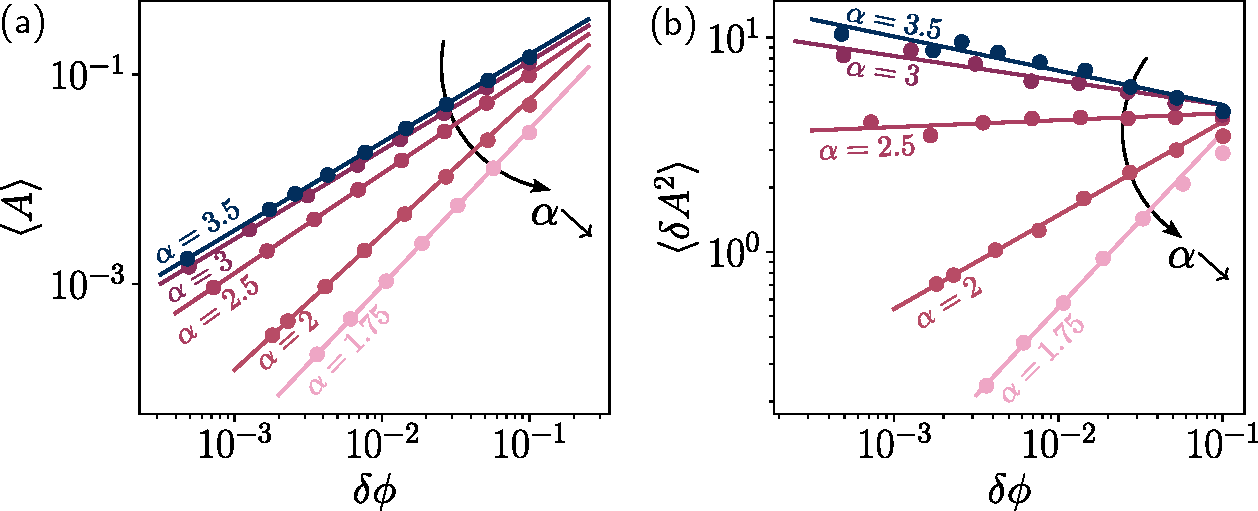
\includegraphics[width=0.9\textwidth]{Chapitre3/Figures/BetaGamma/EvolMeanVar3D_edited.pdf}
	\caption{(a) Évolution de la valeur moyenne de l'activité dans l'état stationnaire $\langle A \rangle$ en fonction de la distance au point critique $\delta\phi$ à différentes portées dans le $\alpha$-ROM en 3D. (b) Idem pour les fluctuations $\langle \delta A^2\rangle = L^D\times(\langle A ^2 \rangle - \langle A \rangle^2)$.}
	\label{fig:evolmeanvar3D}
\end{figure}

\subparagraph{}Par ailleurs, nous retrouvons aussi dans ce cas un point autour duquel la transition change simultanément de convexité et de comportement fluctuant, seulement cette fois localisé en $\alpha\approx 2.5$. En trois dimensions aussi, la criticalité des modèles $\alpha$-ROM est donc très différente associée au cadre LR-CDP. Pour ce qui est du comportement dynamique, l'exposant $\delta$ opère cette fois une évolution quelque peu surprenante. En effet, celui-ci reste constant autour de $\delta \approx 0.74$, valeur associée à la classe CDP à courte portée. Dans cette dimension, les interactions médiées ne semblent donc pas affecter la relaxation vers l'état stationnaire.

\subparagraph{}Finalement, l'étude des modèles $\alpha$-ROM révèle un comportement critique très différent du cadre générique LR-CDP en deux ou trois dimensions. Si l'on retrouve une zone d'exposants $\alpha$ pour lesquels la criticalité dépend continûment de la portée, celle-ci concerne des valeurs de $\alpha$ bien plus petites que dans le cadre canonique. De plus, cette zone d'évolution continue n'est pas bornée par le champ moyen associé à celui de CDP, mais par une limite non-triviale en dimension finie, caractérisée par une convexité et des fluctuations évanescentes. Pourtant, l'évolution continue des exposants passe effectivement par un point caractérisé par les mêmes exposants statiques que le champ moyen CDP. Seulement, dans le cas des interactions médiées, celui-ci ne constitue pas un comportement limite. Les interactions médiées constituent donc un mécanisme permettant d'aller au-delà du champ moyen associé au comportement de courte portée, laissant place à un comportement exotique $\beta >1$, $\gamma^\prime<0$ sur toute une gamme de portées $\alpha$ physiquement envisageables.

\subsection{Hyperuniformité}

\label{sec:TBLRRHU}

\subparagraph{}Une autre manière de caractériser le modèle $\alpha$-ROM est de s'intéresser aux propriétés de structure à la transition. Dans le \autoref{chapter:introduction}, nous avons vu que proche du point critique, les modèles dans la classe CDP présentent un phénomène d'hyperuniformité. Dans le \autoref{chapter:TransportLP}, nous avons vu que dans le cadre LR-CDP, la propriété d'hyperuniformité est modifiée par la présence de transport à longue portée induit localement par l'activité. Notamment, l'exposant $\alpha_\text{HU}$ caractérisant l'évolution du facteur de structure selon $S(\mathbf{q})\sim q^{\alpha_\text{HU}}$ évolue continûment de $\alpha_\text{HU}^\text{CDP, 2D}\approx 0.5$ à $\alpha_\text{HU}^\text{CDP, CM} = 0$ dans la zone $3<\alpha<4$ en 2D. L'hyperuniformité est donc perdue à longue portée dans ce cas. Les exposants critiques $\beta$, $\gamma^\prime$ et $\delta$ suivant une évolution différente du cadre LR-CDP dans le cas des interactions médiées à longue portée considérées dans le $\alpha$-ROM, il est naturel de se demander s'il en va de même pour l'exposant d'hyperuniformité. En d'autres termes, l'hyperuniformité est-elle aussi perdue dans la limite de longue portée des interactions hydrodynamiques ? 

\subparagraph{}En réalité, cette question a déjà été abordée par Mari et al. \cite{mari_absorbing_2022} lors de l'étude du 0-ROM. Dans ce cas de portée infinie, les auteurs ont montré que l'hyperuniformité est effectivement perdue à grande échelle. La question restante est alors de savoir comment s'opère ce changement de propriété avec l'évolution de la portée des interactions. Dans cette sous-section, nous nous basons sur des observations qualitatives pour fournir un début de réponse à cette question.

\subsubsection{Méthode}

\subparagraph{}Pour ce faire, nous utilisons, en plus de la méthode de box-counting présentée à la \autoref{sec:HUjumps}, une mesure du facteur de structure $S(\mathbf{q})$. Afin de rendre son calcul efficace pour de petites valeurs de q (i.e., à des échelles spatiales grandes devant la taille des particules), nous définissons un équivalent du champ de densité $\rho(\mathbf{r}_i)$ sur le réseau discret de pas $D_p$, utilisé pour calculer les interactions actives-passives. Dans chaque case située autour de $\mathbf{r}_i$, $\rho(\mathbf{r}_i)$ prend alors une valeur entière correspondant aux nombres de particules présentes dans cette case. Ce faisant, nous pouvons donc utiliser les algorithmes de FFT pour calculer $\hat{\rho}(\mathbf{q}_i)$ dans l'espace réciproque discret et on a alors :

\begin{equation}
	S(\mathbf{q}_i) = \langle|\hat{\rho}(\mathbf{q}_i)|^2\rangle
\end{equation}

\noindent avec $\langle \cdot \rangle$ définissant une moyenne sur différentes réalisations du système dans des conditions équivalentes. Pour évaluer l'évolution de $S(\mathbf{q})$ avec la norme du vecteur d'onde $q$ et donc sonder son évolution à petits $q$, nous réalisons une moyenne isotrope dans l'espace réciproque. En pratique, chaque point $S(q)$ est calculé par une moyenne sur l'anneau d'épaisseur $\frac{2\pi}{L}$ associé dans l'espace réciproque.

\subparagraph{}Afin de pouvoir comparer les répartitions de densité pour les différentes portées $\alpha$, nous nous plaçons à une distance fixée du point critique $\delta\phi \approx 1\times 10^{-2}$. Ce critère est en effet essentiel pour la comparaison puisque, comme nous l'avons vu au \autoref{chapter:TransportLP}, les propriétés d'hyperuniformité dépendent de la distance au point critique. Notamment, la propriété d'hyperuniformité est perdue à grande échelle pour des distances $\delta\phi$ trop grandes. Cette distance fixée est alors choisie de telle façon que les simulations associées à chaque portée puissent se dérouler sur des temps raisonnables ($<24~\text{h}$ pour une simulation individuelle). Afin d'obtenir une meilleure statistique, nous moyennons ces mesures sur plusieurs dizaines de configurations indépendantes dans l'état stationnaire. Les résultats obtenus sont alors représentés sur la \autoref{fig:HUTBLRR}-(a). En parallèle, les mesures de type box-counting sont effectuées et les résultats associés sont représentés sur la \autoref{fig:HUTBLRR}-(b).

\subsubsection{Résultats}

\begin{figure}[h]
	\centering
	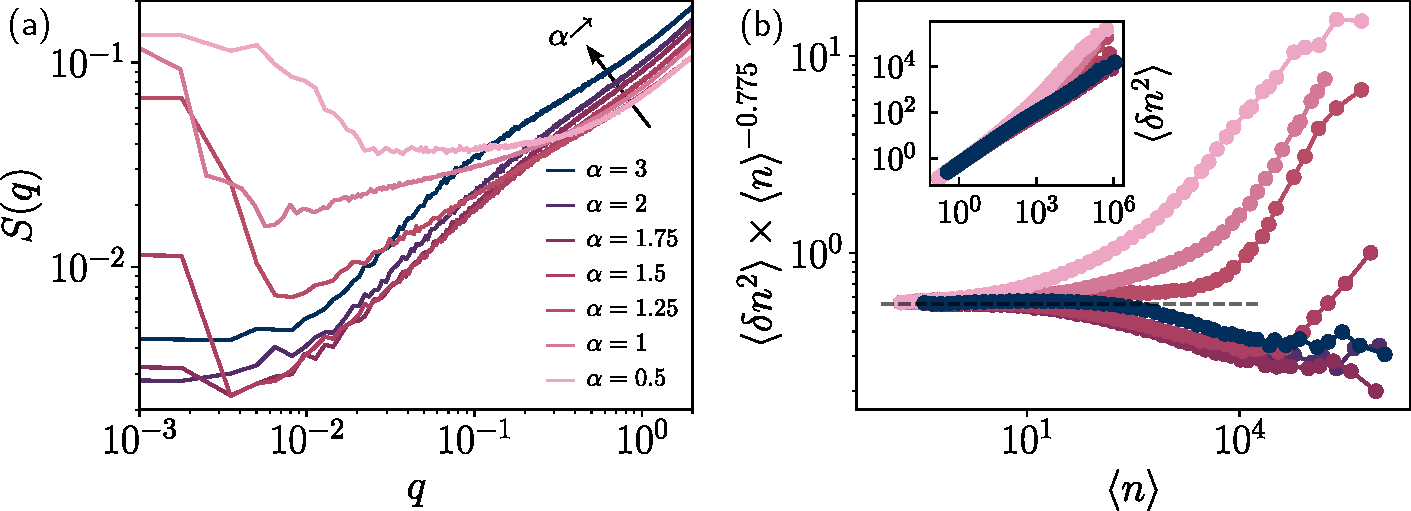
\includegraphics[width=\textwidth]{Chapitre3/Figures/HU/HUTBLRR.pdf}
	\caption{Hyperuniformité dans le modèle $\alpha$-ROM en 2D à $\delta\phi \approx 1\times 10^{-2}$. (a) Évolution du facteur de structure isotrope avec le nombre d'onde. (b) Méthode box-counting (voir \autoref{sec:HUjumps}) compensée par le comportement mesuré à courte portée $\alpha = 3$. En encart, les données brutes.}
	\label{fig:HUTBLRR}
\end{figure}

\subparagraph{}Dans la limite de longue portée $\alpha = 0.5$, nous retrouvons les résultats de Mari et al. \cite{mari_absorbing_2022} avec une perte du caractère évanescent de $S(\mathbf{q})$ à petits $q$. Dans la limite de courte portée $\alpha = 3$, l'allure globale de la courbe présente bien une diminution de $S(\mathbf{q})$ à petits $q$ bien que celle-ci ne semble pas suivre une loi de puissance évidente et sature à très petits $q$. Cette saturation peut notamment s'expliquer par la distance finie au point critique examinée. L'observation de cette évanescence marque alors une forte différence avec le cas LR-CDP. En effet, dans ce cas, l'hyperuniformité est déjà complètement perdue à cette valeur de $\alpha$.  

\subparagraph{}Entre ces deux extrémités, les portées intermédiaires montrent une évolution intéressante. Si pour $\alpha > 1.5$ les facteurs de structure sont difficilement distinguables, pour $\alpha \leq 1.5$ leur évolution montrent d'abord une décroissance plus faible à des valeurs de $q$ intermédiaires puis une augmentation à très petits $q$. Cette évolution suggère alors une perte de l'hyperuniformité à grande échelle dans le régime critique.

\subparagraph{}Un aspect de notre comparaison des différentes portées peut être questionné. Nous pouvons en fait imaginer deux façons de définir la distance à la transition, qui doit être fixée pour comparer les résultats obtenus pour différents $\alpha$. Ici, nous avons fait le choix de la caractériser via $\delta\phi$, qui est le choix le plus standard. Une autre possibilité aurait été de la caractériser via la valeur moyenne de l'activité dans l'état stationnaire $\langle A \rangle$. Dans ce cas, sachant que la convexité de la transition augmente avec la portée des interactions, nous en conclurions que les données présentées pour les plus petites valeurs de $\alpha$ sont bien plus proches de la transition que celles présentées pour les  plus grandes valeurs de $\alpha$. Pourtant, nous mesurons ici une perte du caractère hyperuniforme dans le cas des plus petites valeurs de $\alpha$. Sachant que l'on attend que les propriétés hyperuniformes se développent d'autant plus que le système est proche de la transition, un changement de convention pour définir la distance à la transition ne permettrait donc pas de renverser la tendance observée ici, il l'exacerberait plutôt.

\subparagraph{}Cette tendance est moins évidente  mais se retrouve qualitativement dans le cas de la méthode de box-counting. En compensant l'évolution de $\langle \delta n^2 \rangle$ avec l'évolution mesurée à très courte portée $\langle \delta n^2 \rangle \sim \langle n \rangle^{0.775}$ sur la \autoref{fig:HUTBLRR}-(b), les évolutions pour $\alpha<1.5$ semblent aussi contraster avec celles de plus courtes portées $\alpha>1.5$, révélant un comportement localement "moins hyperuniforme" (i.e. un exposant effectif local $\sigma^\text{eff}$ plus grand).

\subparagraph{}Finalement, cette analyse qualitative des propriétés d'hyperuniformité du $\alpha$-ROM semble montrer un changement autour de $\alpha = 1.5$. Pour $\alpha<1.5$, les observations suggèrent une hyperuniformité perdue à grande échelle. De la même manière que le transport à longue portée induit localement par l'activité, les interactions médiées effacent donc le caractère hyperuniforme de la transition. Toutefois, la zone d'effet $\alpha < 1.5$ qualitativement identifiable ici est à nouveau très différente de celle prévue par le cadre de référence LR-CDP pour lequel on a $\alpha<3$. Une étude plus approfondie serait cependant nécessaire pour confirmer ces premières observations.

\subsection{Retour sur les cas physiques}

\subparagraph{}Au début de ce chapitre, nous avions identifié deux cas de portée pertinents dans le cadre de la transition de réversibilité des suspensions cisaillées cycliquement. Le premier, similaire au cas de l'expérience de Pine et. al \cite{pine_chaos_2005}, a lieu dans un milieu 3D peu confinant. Dans notre modélisation stroboscopique cela revient à $\alpha = 2$ dans le $\alpha$-ROM en 3D. Les résultats présentés au cours de cette section placent ce cas au cœur de la zone d'évolution continue des exposants avec $\beta > 1$ et $\gamma^\prime < 0$. La transition attendue est donc convexe.

\subparagraph{}Le second cas pertinent est le cas d'un cisaillement confiné entre deux plaques rigides, pour lequel on a $\alpha = 3$ dans un milieu quasi-2D. Notre étude du $\alpha$-ROM en 2D place alors cette situation dans la limite de courte portée, dans laquelle la transition adopte le comportement de la classe CDP, soit concave, avec des fluctuations qui divergent et des propriétés hyperuniformes. Ainsi, notre analyse indique que l'influence des interactions médiées à longue portée dépend fortement du système réel étudié, celles-ci n'ayant un impact sur le comportement critique que dans certains cas.

\subsection*{Bilan}

\subparagraph{}Finalement, l'analyse des propriétés statiques (\autoref{sec:TBLRRStat}), dynamiques (\autoref{sec:TBLRRdyn}) et de structure (\autoref{sec:TBLRRHU}) des transitions du $\alpha$-ROM montre que les interactions médiées dans ce système agissent sur le comportement critique d'une manière originale. Notamment l'évolution des exposant critiques avec l'exposant de portée $\alpha$ ne peut pas être comprise dans le cadre LR-CDP qui représente l'influence de sauts à longue portée dans le système. Plus particulièrement, nous observons une large gamme de portées en 2D et en 3D montrant un comportement convexe de la transition et évanescent des fluctuations. Ces observations n'étant pas rationalisables dans le cadre LR-CDP, il semble que la diffusion des particules passives dans le modèle constitue un mécanisme dont l'appréhension nécessite un nouveau cadre théorique.

\section{Interprétation}

\label{sec:interpret}

\subparagraph{}Que ce soit dans le cas du ROM appartenant à la classe CDP ou dans le cas du LR-ROM rattaché au cadre LR-CDP, la dynamique du système est contrôlée par le transport des particules actives (et donc transport induit localement par l'activité). Comme nous l'avons détaillé dans la section précédente, ce mécanisme, par les cadres théoriques qu'il appelle, ne permet pas d'appréhender la criticalité dans les modèles $\alpha$-ROM.

\subparagraph{}Comme nous l'avons déjà évoqué au \autoref{chapter:introduction}, nous pensons que cette distinction est due à la nature des interactions à longue portée dans ces modèles. Celles-ci n'induisent en fait pas un transport des particules induit localement par l'activité mais plutôt un bruit interne induit non-localement par l'activité auquel sont soumises l'ensemble des particules du système. Au niveau de l'implémentation numérique de notre modèle, ce bruit interne est représenté par le processus diffusif composé de la succession des petits déplacements $\boldsymbol\delta^p$ (voir \autoref{fig:modelsusp}). Ce mécanisme propose alors un nouveau mode de création d'activité par rapport au ROM et au LR-ROM : deux particules passives peuvent devenir actives en se recouvrant après diffusion. Là où le processus de propagation de l'activité par transport des particules actives (toujours présent dans le $\alpha$-ROM) est représenté par le processus de réaction-diffusion $A +B \xrightarrow[]{\lambda} 2A$ (voir \autoref{sec:CompCDP}), on pourrait formellement représenter ce nouveau mode de création de l'activité par l'équation :

\begin{equation}
	B +B \xrightarrow[]{} A + A
	\label{eq:meca_diff}
\end{equation}

\noindent les particules passives représentées par l'espèce $B$ ayant une dynamique stochastique dictée non-localement par l'espèce $A$. Nous pensons que c'est l'ajout de cette seconde réaction qui rend le comportement critique du $\alpha$-ROM très différent du cadre LR-CDP.

\subparagraph{}Dans ce chapitre, nous proposons un cadre d'interprétation de la transition de réversibilité dans les suspensions cisaillées cycliquement suivant ces lignes. Pour ce faire, nous partirons du modèle de Hébraud-Lequeux, incontournable dans le cas de la transition vers l'écoulement des fluides à seuil, pour développer un modèle champ moyen associé au $\alpha$-ROM. Se construisant via la notion de bruit interne, ce modèle permettra de mettre en évidence le mécanisme diffusif induit non-localement comme origine de la convexité des transitions précédemment caractérisées.

\subparagraph{}Nous généraliserons ensuite ce cadre champ moyen pour obtenir une première compréhension de  l'effet de la longue portée des interactions sur le processus diffusif et le comportement critique résultant. Cette analyse mènera à l'établissement d'un cadre théorique, alternative au cadre LR-CDP, qui nous permettra une première interprétation des résultats présentés dans la section précédente. 

\subparagraph{}Enfin, via des modifications de notre modèle numérique et des mesures complémentaires, nous mettrons en évidence les limites mais aussi les apports de cette approche de champ moyen pour interpréter la criticalité des modèles $\alpha$-ROM.

\subsection{Un cadre de description champ moyen}

\subparagraph{}Dans le cadre de la transition vers l'écoulement des fluides à seuil, la présence d'un bruit mécanique issu des interactions à longue portée médiées par le milieu a fait l'objet de diverses études \cite{lin_mean-field_2016, ferrero_criticality_2019}. D'un point de vue champ moyen, cette interprétation permet d'établir un modèle permettant de rendre compte de la convexité de la transition observée expérimentalement. Ce modèle est le modèle de Hébraud-Lequeux\cite{hebraud_mode-coupling_1998}, que l'on présentera plus spécifiquement à la \autoref{sec:HL_def} du \autoref{chapter:yielding}. Du fait des similarités entre les transitions de réversibilité et d'écoulement présentées au \autoref{chapter:introduction}, notamment la présence d'un bruit interne, nous cherchons dans cette partie à définir un modèle équivalent au modèle Hébraud-Lequeux dans le cas de la transition de réversibilité afin de rendre compte des convexités mesurées dans la section précédente.

\subparagraph{}Pour ce faire, nous présenterons d'abord l'image champ moyen permettant d'établir un tel modèle. Nous montrerons alors que si celui-ci est très proche du modèle original de Hébraud-Lequeux, il existe entre ces deux formulations certaines différences. Malgré cela, nous montrerons par une résolution analytique que ce cadre d'interprétation champ moyen permet effectivement de décrire une transition convexe dans le cadre de la transition de réversibilité. Toujours inspiré du cadre de la transition vers l'écoulement, nous mettrons alors ce modèle à profit pour interpréter l'effet de la portée des interactions sur le comportement critique observé dans le $\alpha$-ROM.

\subsubsection{Première modélisation et diffusion normale}

\label{sec:diffnorm}

\paragraph{Présentation du modèle}

\subparagraph{}La philosophie du modèle de Hébraud-Lequeux capturant l'effet du bruit interne dans la transition vers l'écoulement consiste à se concentrer sur la dynamique effective d'un agent unique du système, diffusant vers une barrière sous l'action de l'activité globale. Nous proposons une image s'adaptant à cette formulation dans le cadre de la dynamique des particules dans le $\alpha$-ROM, illustrée à la \autoref{fig:LHLmodel}.

\subparagraph{}Considérons une particule passive dans notre modèle numérique. Au cours du temps, celle-ci diffuse jusqu'à rencontrer une autre particule. Dans une approche champ moyen négligeant toutes corrélations  (d'activité, de positions, ...), nous pouvons représenter les particules entourant notre particule d'intérêt par une cage effective de rayon $R$. En supposant une répartition des particules uniforme dans le système, la taille de cette cage peut être directement associée à la distance interparticulaire typique $l$ et donc à la densité de particules $\phi$. On a alors $R\sim \phi^{-1/D}$. En centrant cette zone de piégeage sur l'origine du repère, la particule cible positionnée en $\mathbf{r}$ peut donc prendre deux états : passive si elle n'entre pas en contact avec d'autres particules ($|\mathbf{r}|<R$), et active si elle sort de la cage effective ($|\mathbf{r}|>R$). 

\begin{figure}[h]
	\centering
	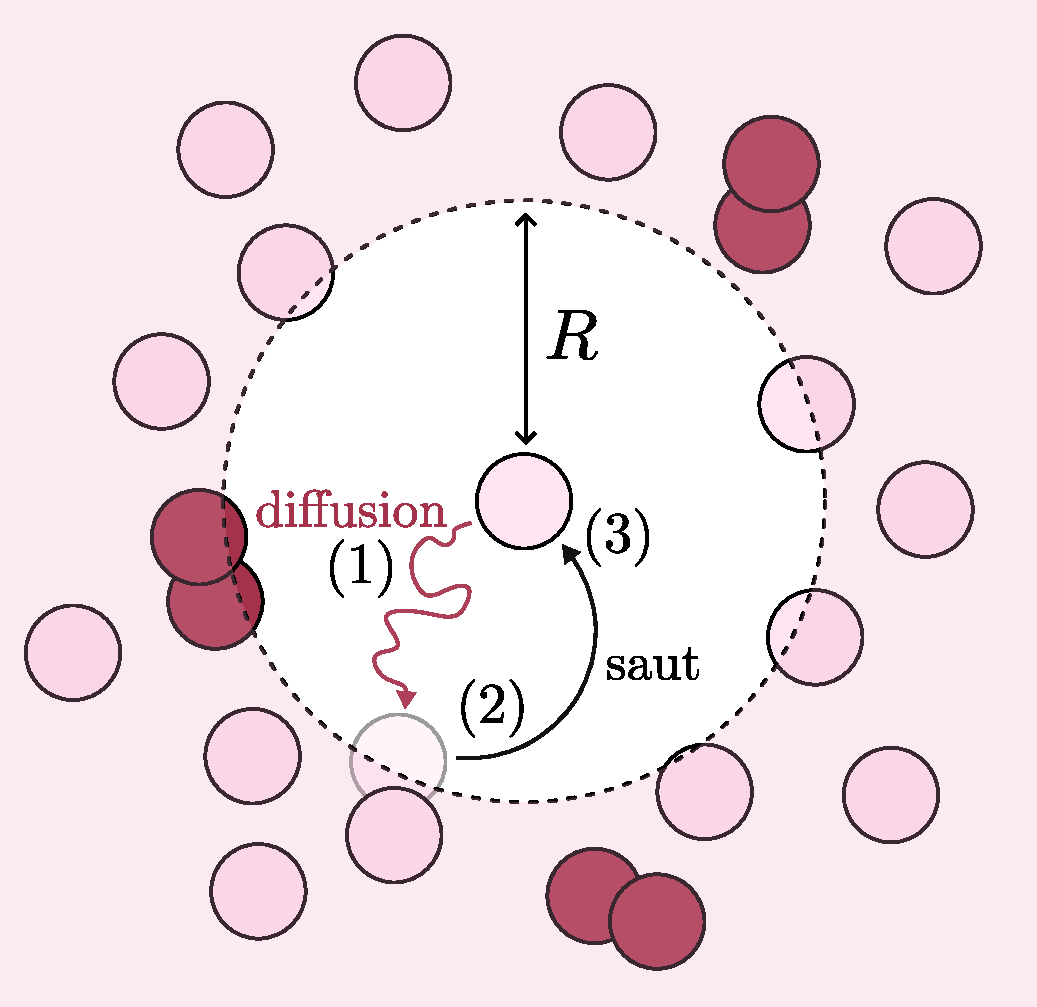
\includegraphics[width=0.5\textwidth]{Chapitre3/Figures/Interpretation/LHLModel.pdf}
	\caption{Représentation champ moyen de la dynamique du $\alpha$-ROM.}
	\label{fig:LHLmodel}
\end{figure}

\subparagraph{}Lorsque la particule est passive, celle-ci est soumise à un bruit interne dont l'intensité est proportionnelle au nombre de particules actives dans l'environnement (i.e. l'activité dans le système). Dans cette vision statistique du problème où toutes les particules ont une dynamique équivalente, cette intensité du bruit est proportionnelle à la probabilité (notée $\Gamma\tau$ dans la suite) pour la particule d'être active. En première intention de modélisation, nous considérons ce bruit comme gaussien et donc que la particule diffuse avec un coefficient de diffusion $D=a\Gamma$ sous l'action de l'activité globale. En pratique, cette modélisation correspond donc à une portée infinie ($\alpha = 0$) du propagateur d'interaction dans le modèle microscopique, comme proposé dans le modèle de Mari et al. \cite{mari_absorbing_2022}.

\subparagraph{}Lorsque la particule est active, elle effectue un saut, comme dans le $\alpha$-ROM, sur un temps typique $\tau$. Dans notre modélisation champ moyen, nous considérons ce saut suffisamment grand pour replacer la particule à l'origine d'une nouvelle cage effective, la rendant de nouveau passive. 

\subparagraph{}Dans cette image simple, nous pouvons modéliser l'évolution de la distribution de probabilité $P(\mathbf{r})$ de la position $\mathbf{r}$ de la particule par les équations suivantes :

\begin{equation}
\begin{aligned}
    \partial_t P(\mathbf{r}, t) &= a\Gamma (t)\nabla^2 P(\mathbf{r}, t) - \frac{1}{\tau}\Theta(|\mathbf{r}|>R)P(\mathbf{r}, t) + \delta(\mathbf{r})\Gamma (t)\\ \Gamma (t) &= \frac{1}{\tau}\int_{|\mathbf{r}|>R}\mathrm{d}\mathbf{r}~P(\mathbf{r}, t)
    \label{eq:muHLDiff}
\end{aligned}
\end{equation} 

\noindent avec $a$ un paramètre réel positif. Le premier terme du membre de droite représente la diffusion de la particule ((1) sur la \autoref{fig:LHLmodel}), le second le processus de saut actif ((2) sur la \autoref{fig:LHLmodel}) et le troisième l'apparition dans une nouvelle cage placée par convention en $\mathbf{r}=0$ ((3) sur la \autoref{fig:LHLmodel}). 

\subparagraph{}Comme nous le montrons juste après via sa résolution numérique, le modèle ainsi défini présente une transition de phase absorbante de paramètre d'ordre $\Gamma = \langle \Gamma (t) \rangle$ et de paramètre de contrôle $R$. Ces deux quantités sont les pendants directs de l'activité $\langle A \rangle$ et de la densité\footnote{Nous rappelons que dans notre modélisation champ moyen $R\sim \phi^{-1/D}$.} $\phi$ dans le $\alpha$-ROM.


\paragraph{Comparaison avec la formulation originale}

\subparagraph{}Le modèle défini par cette image champ moyen dans le modèle de particules ressemble fortement au modèle de Hébraud-Lequeux utilisé dans le cadre de la transition vers l'écoulement (voir \autoref{sec:HL_def}). Dans ce cas où la variable d'intérêt est une contrainte locale $\sigma$ et non la position d'un objet, les équations prennent en fait la forme suivante :

\begin{equation}
\begin{aligned}
    \partial_t P(\sigma, t) &= -\dot{\gamma}\partial_\sigma P(\sigma, t)+a\Gamma (t)\partial_\sigma^2 P(\sigma, t) - \frac{1}{\tau}\Theta(|\sigma|>\sigma_Y)P(\sigma, t) + \delta(\sigma)\Gamma (t)\\
    \Gamma (t) &= \frac{1}{\tau}\int_{|\sigma|>\sigma_Y}\mathrm{d}\sigma~P(\sigma, t)
\end{aligned}
\label{eq:HL_comp}
\end{equation} 

\subparagraph{} On peut cependant remarquer deux différences principales entre ces deux formulations. La première est que la diffusion prend place dans un espace de dimension 1 dans le cadre de la transition vers l'écoulement alors qu'elle prend place dans un espace de dimension 2 ou 3 pour le modèle de suspensions. La seconde est la présence d'un terme additionnel dans l'\autoref{eq:HL_comp}, le premier du membre de droite. Ce terme en dérivée première de la distribution correspond à un forçage du système. Absent dans le cas du modèle de suspensions, il biaise la diffusion de la variable vers la barrière. Dans le cas de la transition de réversibilité, celui-ci reviendrait à l'ajout d'un mécanisme déterministe d'attraction vers le bord de la cage.

\subparagraph{}Cette seconde différence introduit une autre différence plus fondamentale. Dans le cas du modèle de Hébraud-Lequeux, le paramètre de contrôle habituel n'est pas $\sigma_Y$ (et donc de manière équivalente $R$ dans le cas des suspensions) mais plutôt la valeur moyenne de la variable d'intérêt $\Sigma = \int \mathrm{d}\sigma~\sigma P(\sigma,t)$. En effet, dans ce cas, via la brisure de symétrie opérée par le terme additionnel, celle-ci n'est plus nulle. La phénoménologie de la transition associée est donc décrite par la relation :

\begin{equation}
	\Gamma \sim (\Sigma - \Sigma_c)^\beta
	\label{eq:paramordre_HL}
\end{equation}

\subparagraph{}Dans le cadre du modèle d'écoulement, la résolution numérique de ce modèle donne $\beta=2$ et permet donc d'expliquer la convexité de la transition via le mécanisme de diffusion sous l'activité globale. On peut alors se demander si ce résultat tient toujours dans la formulation champ moyen adaptée au modèle de suspensions, malgré les deux différences mises en évidence dans cette partie.

\paragraph{Résolution en 2D}

\subparagraph{}Afin de montrer que ce modèle champ moyen permet effectivement de retrouver une transition convexe par ce mécanisme de diffusion, nous le résolvons en deux dimensions pour déterminer la relation $\Gamma \sim (R - R_c)^\beta$ à petits $\Gamma$. Pour ce faire, nous commençons par adimensionner l'\autoref{eq:muHLDiff} par les transformations :

\begin{equation}
	\tilde{t} = \frac{t}{\tau}, \quad \tilde{\mathbf{r}} = \frac{\mathbf{r}}{R}
\end{equation}

\noindent En nous plaçant de plus dans l'état stationnaire, nous obtenons alors :

\begin{equation}
    0 = \tilde{a}\tilde{\Gamma}\tilde{\nabla}^2 P(\tilde{\mathbf{r}}) - \Theta(|\tilde{\mathbf{r}}|>1)P(\tilde{\mathbf{r}}) + \delta(\tilde{\mathbf{r}})\tilde{\Gamma}, \quad \tilde{\Gamma} = \int_{|\tilde{\mathbf{r}}|>1}\mathrm{d}\tilde{\mathbf{r}}~P(\tilde{\mathbf{r}}),\quad \tilde{a} = \frac{a}{R^2}
\end{equation} 

\noindent Dans la suite de la résolution, nous omettrons les $\tilde{}$ pour alléger les notations. Sous cette transformation, le paramètre de contrôle est $a$, relié à la densité de particules via $a\sim \phi$ puisque nous rappelons que l'on a $R\sim 1/\sqrt{\phi}$ en 2D.

\subparagraph{}Nous résolvons ensuite cette équation par morceaux dans les domaines disjoints $r<1$ (zone I) et $r>1$ (zone II). Dans la zone I, la résolution donne :

\begin{equation}
	P_\text{I}(\mathbf{r}) = c_1 \ln (r) + c_2, \quad (c_1, c_2) \in \mathbb{R}^2
\end{equation}

\noindent et dans la zone II :

\begin{equation}
	P_\text{II}(\mathbf{r}) = c_3 K_0\left( \frac{r}{\sqrt{a\Gamma}} \right), \quad c_3 \in \mathbb{R}
\end{equation}

\noindent avec $K_0$ la fonction de Bessel modifiée de seconde espèce d'ordre 0 \cite{abramowitz_handbook_1965}. La distribution $P(\mathbf{r})$ étant continue et de dérivée continue en $r=1$, on obtient finalement :

\begin{equation}
P(\mathbf{r}) = \left\{
    \begin{aligned}
    & c_3 \left( K_0\left( \frac{1}{\sqrt{a\Gamma}} \right) -K_1\left( \frac{1}{\sqrt{a\Gamma}} \right)\frac{\ln (r)}{\sqrt{a\Gamma}}\right), \quad r<1\\
    & c_3 K_0\left( \frac{r}{\sqrt{a\Gamma}} \right), \quad r>1
    \end{aligned}
    \right.
\end{equation}

\subparagraph{}La condition de normalisation de la distribution permet alors de déterminer la constante $c_3$. En effet on a :

\begin{equation}
	I_\text{I} = \int_0^1 \mathrm{d}r~ 2\pi r P(\mathbf{r}) = \pi c_3 K_0\left( \frac{1}{\sqrt{a\Gamma}} \right) + \frac{\pi c_3}{2\sqrt{a\Gamma}}K_1\left( \frac{1}{\sqrt{a\Gamma}} \right)
\end{equation}

\begin{equation}
	I_\text{II} = \int_0^\infty \mathrm{d}r~ 2\pi r P(\mathbf{r}) = 2\pi c_3 \sqrt{a\Gamma}K_1\left( \frac{1}{\sqrt{a\Gamma}} \right)
\end{equation}

\noindent en utilisant la propriété $(z^\nu K_\nu (z))^\prime = -z^\nu K_{\nu-1}(z)$. Nous obtenons alors :

\begin{equation}
\frac{1}{c_3} = \pi K_0\left( \frac{1}{\sqrt{a\Gamma}} \right) + \frac{\pi}{2\sqrt{a\Gamma}}K_1\left( \frac{1}{\sqrt{a\Gamma}} \right)+2\pi \sqrt{a\Gamma}K_1\left( \frac{1}{\sqrt{a\Gamma}} \right)
\end{equation}

\subparagraph{}La valeur de $\Gamma$ dans l'état stationnaire est alors donnée par la relation d'auto-cohérence :

\begin{equation}
	\Gamma = \frac{2\pi \sqrt{a\Gamma}K_1\left( \frac{1}{\sqrt{a\Gamma}} \right)}{\pi K_0\left( \frac{1}{\sqrt{a\Gamma}} \right) + \frac{\pi}{2\sqrt{a\Gamma}}K_1\left( \frac{1}{\sqrt{a\Gamma}} \right)+2\pi \sqrt{a\Gamma}K_1\left( \frac{1}{\sqrt{a\Gamma}} \right)}
	\label{eq:blabla}
\end{equation}

\noindent Étant intéressés par le comportement asymptotique à petit $\Gamma$, nous développons les fonctions de Bessel asymptotiquement selon \cite{abramowitz_handbook_1965} :

\begin{equation}
	K_\nu (x) \sim \sqrt{\frac{\pi}{2x}}e^{-x}\left( 1+\frac{4\nu^2-1}{8x}+\mathcal{O}(1/x^2) \right)
\end{equation}

\noindent En développant le membre de droite de l'\autoref{eq:blabla} au premier ordre non-trivial nous obtenons finalement :

\begin{equation}
	\Gamma = 4a\Gamma\left( 1-2\sqrt{a\Gamma}+\mathcal{O}(a\Gamma) \right)
\end{equation}

\noindent Il y a alors deux cas possibles selon la valeur de $a$ et sa comparaison avec la valeur critique $a_c = \frac{1}{4}$. Pour $a<a_c$, la seule solution est $\Gamma = 0$. Pour $a>a_c$, une autre solution $\Gamma > 0$ apparaît, se comportant comme $\Gamma \sim (a-a_c)^2$. Si l'on revient aux variables dimensionnées, cela revient à :

\begin{equation}
	\Gamma \sim (R_c-R)^2
	\label{eq:resolhl2d}
\end{equation}

\subparagraph{}Ainsi, ce modèle rend bien compte d'une transition de phase absorbante avec une phase absorbante $\Gamma = 0$ lorsque la cage effective est suffisamment grande $R>R_c$, et une phase active $\Gamma >0$ lorsque celle-ci est suffisamment petite $R<R_c$. Étant donné que l'on a $R\sim 1/\sqrt{\phi}$ en 2D dans l'image champ moyen et que $\Gamma$ correspond à l'activité dans le système, le comportement qualitatif de transition du $\alpha$-ROM est bien retrouvé. De plus, dans l'image champ moyen celui-ci est donc caractérisé par un exposant critique $\beta = 2$. Ce modèle simple permet donc effectivement de retrouver la convexité de la transition de réversibilité. Les différences entre le modèle champ moyen d'écoulement et celui de réversibilité n'impactent donc pas la criticalité du système.

\subparagraph{}Via ce nouveau cadre de modélisation statistique, nous sommes donc capables d'interpréter la convexité des transitions observées dans le $\alpha$-ROM. Toutefois, cette approche champ moyen ne permet pas de rendre compte de l'évolution de cette convexité avec la portée des interactions associées puisque celles-ci sont encodées dans un terme de bruit gaussien générique, quel que soit $\alpha$. Dans la partie suivante, nous montrons, en suivant les lignes d'études menées sur la transition vers l'écoulement, que l'effet de la portée des interactions peut en fait être introduit dans cette image simple afin de formuler des prédictions quant à l'évolution de l'exposant $\beta$ avec $\alpha$ dans un cadre champ moyen.
 
\subsubsection{Influence de la longue portée et diffusion anormale}

\label{sec:LPHL}

\subparagraph{}Dans le cadre de la transition vers l'écoulement, les auteurs de l'étude \cite{lin_mean-field_2016} ont montré que la modélisation gaussienne du bruit n'était pas toujours la plus pertinente pour décrire l'effet des interactions à longue portée dans le système. Dans cette partie, nous reprenons cet argument pour le transposer au modèle de suspensions.

\paragraph{Interactions à longue portée et distributions de bruit interne}

\subparagraph{}En fait, du fait de la propriété de décroissance algébrique du propagateur hydrodynamique $ \mathcal{G}$, le bruit interne peut être largement distribué. Dans l'image champ moyen développée précédemment, cela revient à considérer que la particule cible effectue des sauts de Lévy de taille $\Delta$ distribuée selon :

\begin{equation}
	P(\Delta) \sim \frac{1}{\Delta^{1+\mu}}
\end{equation}

\noindent avec\footnote{Dans la limite $\mu \geq 2$, la variance de la distribution est finie et donc ce processus se ramène à une marche aléatoire gaussienne.} $\mu < 2$. Dans notre modélisation probabiliste, cela revient donc à modifier l'\autoref{eq:muHLDiff} selon :

\begin{equation}
\begin{aligned}
    \partial_t P(\mathbf{r}, t) &= -a\Gamma (t)|\nabla|^{\mu} P(\mathbf{r}, t) - \frac{1}{\tau}\Theta(|\mathbf{r}|>R)P(\mathbf{r}, t) + \delta(\mathbf{r})\Gamma (t)\\
     \Gamma (t) &= \frac{1}{\tau}\int_{|\mathbf{r}|>R}\mathrm{d}\mathbf{r}~P(\mathbf{r}, t)
\end{aligned}
    \label{eq:muHL}
\end{equation}

\noindent avec $|\nabla|^{\mu}$ l'opérateur de dérivée fractionnaire déjà défini au \autoref{chapter:TransportLP} dans le cadre du transport à longue portée. Celui-ci traduit alors une diffusion anormale de la particule.

\subparagraph{}D'un point de vue champ moyen, nous pouvons déterminer la valeur de $\mu$ en fonction de la portée des interactions hydrodynamiques. Dans le cas où le bruit interne provient d'une unique particule active et où les interactions médiées décrites par le propagateur $\mathcal{G}(\mathbf{r})$ décroissent comme $1/r^\alpha$, la distribution associée est :

\begin{equation}
	P(\Delta) \sim \int \mathrm{d}\mathbf{r}~\delta\left( \mathcal{G}(\mathbf{r})-\Delta \right)\sim \frac{1}{\Delta^{1+D/\alpha}}
\end{equation}

\noindent et on a donc $\mu = D/\alpha$. Ce résultat basé sur un évènement unique reste valable lorsque l'on considère un ensemble de particules actives dans le système, mais à la condition que l'activité dans le système soit totalement décorrélée et n'est donc valable que dans la limite de champ moyen.

\subparagraph{}Nous nommons le modèle généralisé représenté par l'\autoref{eq:muHL}, le modèle $\mu$-Hébraud-Lequeux. Il est alors intéressant de voir comment cette généralisation permet de modifier l'exposant $\beta$ associé en fonction du paramètre $\mu$, afin d'interpréter la dépendance en $\alpha$ observée dans les simulations numériques.

\paragraph{Résultats dans le cadre de la transition vers l'écoulement}

\subparagraph{}La généralisation du modèle de Hébraud-Lequeux à un bruit largement distribué a déjà été étudiée dans le cas de la transition vers l'écoulement. Via cette formulation, les auteurs des études \cite{lin_mean-field_2016, lin_microscopic_2018} sont parvenus à formuler des prédictions sur le comportement critique du modèle en fonction de l'exposant de bruit $\mu$. Dans cette partie, nous rappelons brièvement ces résultats. Ceux-ci sont en fait utiles à notre étude puisque l'on peut penser qu'ils se transposent à notre modèle $\mu$-Hébraud-Lequeux, de la même manière que dans le cas d'une diffusion normale.

\subparagraph{}Par une étude quasistatique de la généralisation de l'\autoref{eq:HL_comp}, il a été montré que l'exposant $\beta$ caractérisant la transition vers l'écoulement via l'\autoref{eq:paramordre_HL} évoluait en fonction de $\mu$ selon :

\begin{equation}
	\beta = \left\{
	\begin{aligned}
	&2, \quad \mu \geq 2\\
	&\mu, \quad 1<\mu\leq2\\
	&1, \quad \mu < 1
	\end{aligned}
	\right.
	\label{eq:PredicBetaLW}
\end{equation}

\noindent retrouvant $\beta = 2$ dans la limite gaussienne et $\beta = 1$ dans la limite $\mu<1$ où la dynamique est dominée par le terme de forçage \cite{lin_mean-field_2016}.

\subparagraph{}Par ailleurs, dans cette même limite d'activité nulle ($P(\sigma>\sigma_Y)=0$), il a été démontré que la distribution $P(\sigma)$ présentait un comportement algébrique proche de la barrière $\sigma = \sigma_Y$ \cite{lin_mean-field_2016} :

\begin{equation}
	P(\sigma_Y-\sigma) \sim (\sigma_Y-\sigma)^\theta
\end{equation}

\noindent avec $\theta$ l'exposant de pseudo-gap. Dans le cas où le système n'est pas forcé, se rapprochant alors du cas de notre modèle de suspensions, il a été montré que cet exposant dépend de l'exposant de bruit $\mu$ selon :

\begin{equation}
	\theta = \left\{
	\begin{aligned}
	&\frac{\mu}{2}, \quad \mu \leq 2\\
	&1, \quad \mu \geq 2
	\end{aligned}
	\right.
	\label{eq:PredicThetaLW}
\end{equation}

\subparagraph{}Le modèle d'écoulement étudié dans \cite{lin_mean-field_2016, lin_microscopic_2018} permet donc de qualifier une évolution de la criticalité de la transition vers l'écoulement en fonction du bruit interne associé. \'Etant très similaire au modèle $\mu$-Hébraud-Lequeux établi dans le cas de la transition de réversibilité, nous nous demandons si nous pouvons transposer ces résultats analytiques à notre cadre d'interprétation champ moyen. En d'autres termes, l'\autoref{eq:PredicBetaLW} et l'\autoref{eq:PredicThetaLW} sont-elles toujours valables dans ce cas ?

\subparagraph{}Dans le cadre de l'image champ moyen que nous avons proposée pour la transition de réversibilité, l'exposant $\beta$ définit la relation entre l'activité $\Gamma$ et la taille de la cage effective $R$ selon :

\begin{equation}
	\Gamma \sim (R_c-R)^\beta
\end{equation}

\noindent Pour ce qui est de l'exposant de pseudo-gap, par transposition, celui-ci définit la relation au point critique :

\begin{equation}
	P(R-|\mathbf{r}|)\sim (R-|\mathbf{r}|)^\theta
\end{equation}

\subparagraph{}Les raisons pour lesquelles cette correspondance de valeur des exposants pourrait ne pas fonctionner sont les différences entre les modèles présentées à la \autoref{sec:diffnorm}, à savoir la différence de dimension et l'existence ou non d'un terme de forçage qui implique un changement du paramètre de contrôle. Toutefois, la correspondance entre les deux modèles dans le cas de la diffusion normale (où l'on trouve $\beta = 2$ dans les deux cas) suggère que ces différences n'impactent pas réellement le comportement critique de la transition. Pour s'en assurer, nous proposons une résolution numérique du modèle $\mu$-Hébraud-Lequeux dans la partie suivante.

\paragraph{Résolution numérique}

\subparagraph{}Afin de confirmer que le modèle $\mu$-Hébraud-Lequeux suit bien le même comportement critique que dans le cas des études \cite{lin_mean-field_2016, lin_microscopic_2018}, nous proposons une résolution de l'\autoref{eq:muHL} par une méthode numérique originale. Celle-ci, détaillée dans l'\annexeref{sec:ResolNumMuHL}, consiste à interpréter cette équation comme une équation de Fokker-Planck généralisée et de la résoudre statistiquement par son équivalent en équation de Langevin avec diffusion anormale. Il est alors possible de déterminer l'évolution de $\Gamma$ avec $R$ et d'en déduire l'exposant critique $\beta$ associé. La méthode de détermination de l'exposant $\beta$ suit alors le même principe que celle dans le cas du $\alpha$-ROM. Les résultats obtenus en 1D et en 2D sont reportés sur la \autoref{fig:LHLNum} où nous avons aussi représenté le comportement prédit dans la théorie homologue pour la transition vers l'écoulement.

\begin{figure}[h]
	\centering
	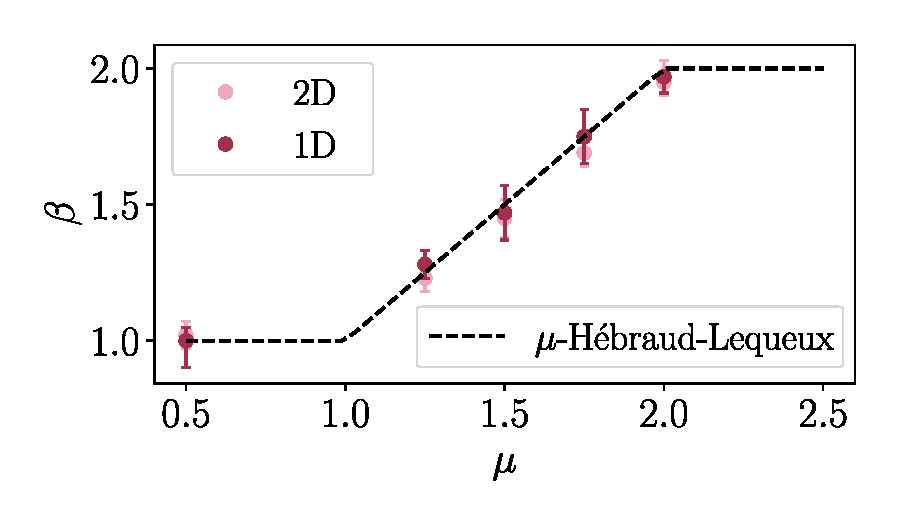
\includegraphics[width=0.6\textwidth]{Chapitre3/Figures/Interpretation/beta_alpha_LevyHL2D.pdf}
	\caption{Évolution de l'exposant $\beta$ mesuré par la résolution numérique de l'\autoref{eq:muHL} en 1D et en 2D (voir \annexeref{sec:ResolNumMuHL}). En pointillés noirs, le comportement du modèle de Lin et al. \cite{lin_microscopic_2018}.}
	\label{fig:LHLNum}
\end{figure}

\subparagraph{}La détermination des exposants n'est pas aisée car elle est coûteuse numériquement, laissant ainsi place à de larges incertitudes de mesure. Toutefois, que ce soit en une ou deux dimensions, les points mesurés montrent un plutôt bon accord avec les prédictions théoriques associées au cadre de la transition vers l'écoulement \cite{lin_microscopic_2018}. Les points en 1D semblent ainsi montrer que l'ajout du terme de forçage ne modifie pas la criticalité de la transition, tandis que les points en 2D suggèrent que cette théorie s'étend trivialement aux dimensions supérieures.

\subparagraph{}Pour la suite de notre analyse nous considérerons donc que le modèle $\mu$-Hébraud-Lequeux suit effectivement une criticalité dictée par l'\autoref{eq:PredicThetaLW} et l'\autoref{eq:PredicBetaLW}. En d'autres termes, dans une gamme d'exposants $1<\mu<2$, la criticalité du modèle dépend continûment de $\mu$ avec $\beta = 2\theta = \mu$. Pour $\mu < 1$, le modèle atteint une limite dans laquelle on a $\beta = 1$ et $\theta = \mu/2$. Pour $\mu>2$, le modèle atteint une limite diffusive dans laquelle nous avons montré que $\beta = 2$, et $\theta = 1$.

\subparagraph{}Le raisonnement présenté à la \autoref{sec:LPHL} implique que $\mu$ est inversement proportionnel à la porté des interactions $\alpha$. Dans le cadre champ moyen représenté par le modèle $\mu$-Hébraud-Lequeux, la portée des interactions semble donc affecter le comportement critique de la même manière que nous l'avons observé dans le $\alpha$-ROM : la convexité de la transition augmente avec la portée. Afin de tester plus spécifiquement cette image champ moyen et sa pertinence pour décrire le mécanisme à l'oeuvre dans les simulations numériques en dimension finie, nous proposons dans la partie suivante un test plus spécifique des prédictions du modèle.


\subsection{Interprétation champ moyen du mécanisme de diffusion dans le $\alpha$-ROM}

\subparagraph{}L'image développée précédemment via le modèle $\mu$-Hébraud-Lequeux est une image champ moyen du mécanisme de diffusion des particules passives et de son influence sur la criticalité de la transition. Puisque champ moyen, elle repose sur deux approximations essentielles : celle que la dynamique des particules actives est décorrélée et celle que la dynamique des particules passives l'est aussi. Dans ce cas, il est possible de faire un lien entre les différents exposants caractérisant le problème.

\subparagraph{}Le premier lien réside dans la relation reliant la portée des interactions caractérisée par l'exposant $\alpha$ et la distribution du bruit interne caractérisée par l'exposant $\mu$. Dans le cas d'une dynamique des particules actives décorrélée, nous avons en effet $\mu = D/\alpha$ comme nous l'avons montré à la \autoref{sec:LPHL}. Le second lien réside dans l'influence de cet exposant $\mu$ sur la criticalité du modèle caractérisée par les exposants $\beta$ et $\theta$. Celui-ci est représenté par l'\autoref{eq:PredicThetaLW} et l'\autoref{eq:PredicBetaLW}. Notamment, pour $1<\mu<2$, nous avons $\beta = \mu$ et $2\theta = \mu$ et donc $\beta = 2\theta$. 

\subparagraph{}Dans cette partie, nous cherchons à tester la pertinence de cette image champ moyen pour interpréter les transitions observées dans le $\alpha$-ROM. La difficulté est que le $\alpha$-ROM est un modèle numérique complexe. Pour deux raisons principales, nous nous attendons d'emblée à ce que celui-ci se démarque de l'image champ moyen. La première raison est que celui-ci fait intervenir deux mécanismes différents pour la création d'activité, comme nous l'avons mentionné au début de cette section. Le premier mécanisme est celui de la diffusion des particules passives induit non-localement par l'activité et le second est celui du transport des particules actives. Par sa construction, le modèle $\mu$-Hébraud-Lequeux basé uniquement sur ce premier mécanisme ne prétend donc pas représenter la criticalité complète du $\alpha$-ROM mais seulement un aspect de celle-ci. La seconde raison est que le $\alpha$-ROM présente une dynamique des particules passives et actives en dimension finie, et donc a priori non exempte de corrélations. 

\subparagraph{}Afin de déterminer si le modèle $\mu$-Hébraud-Lequeux est un cadre d'interprétation pertinent, nous ne pouvons donc pas nous réduire à une comparaison de ses prédictions avec les résultats directement obtenus dans le cadre du $\alpha$-ROM. \`A la place, nous proposons d'étudier la validité de ces prédictions dans des limites du modèle $\alpha$-ROM où les points de divergence conceptuels s'estompent. Si dans la limite où les hypothèses de l'image champ moyen sont satisfaites nous retrouvons les prédictions associées au modèle $\mu$-Hébraud-Lequeux, cela suggère que celui-ci permet bien de représenter le mécanisme de diffusion du $\alpha$-ROM dans son aspect champ moyen.

\subsubsection{Image champ moyen dans une dynamique d'activité décorrélée}

\paragraph{Approche du champ moyen par les grandes dimensions}

\subparagraph{}Afin de pouvoir tester la validité de l'image proposée par le modèle $\mu$-Hébraud-Lequeux, nous proposons donc d'isoler le mécanisme de création de l'activité par diffusion des particules passives dans le $\alpha$-ROM et de le considérer dans sa version champ moyen. 

\subparagraph{}Pour ce faire, nous modifions d'abord le modèle en changeant la dynamique des particules actives. Au lieu de faire des sauts finis, nous considérons cette fois que celles-ci sont redistribuées aléatoirement dans l'espace. Avec les conditions périodiques adoptées, cela équivaut donc à faire des sauts de taille infinie. De ce fait, en accord avec les résultats du \autoref{chapter:TransportLP}, la dynamique d'activité devient champ moyen. Cela permet deux choses : isoler l'influence du mécanisme de diffusion puisque c'est dans ce cas-là le seul capable de produire une criticalité non-triviale, et supprimer les corrélations dans la dynamique d'activité qui pourraient modifier la relation simple $\mu = D/\alpha$ dans le cadre de ce mécanisme.

\subparagraph{}Après cette première modification, il subsiste une source de complexité dans le système, liée à la diffusion des particules passives dans un espace de dimension finie. Pour rendre champ moyen le mécanisme de diffusion des particules passives, nous proposons de supprimer les corrélations dans leur dynamique en considérant des dimensions élevées du système. Ce choix s'explique par le fait que, si comme dans le cas des particules actives nous considérons des particules passives faisant des sauts de taille infinie pour décorréler leur dynamique, le mécanisme de création de l'activité par diffusion serait complètement perdu (puisqu'il ne s'agirait alors plus d'une diffusion). Dans cette limite, nous nous attendons à ce que cette version modifiée du $\alpha$-ROM représente le cadre champ moyen associé au modèle $\mu$-Hébraud-Lequeux. Nous proposons alors, pour tester l'image champ moyen, de mesurer l'exposant $\beta$ dans ce modèle numérique pour la valeur de portée des interactions $\alpha = 0$ et pour les dimensions $D\in\{2,3,4,6\}$. Si le cadre $\mu$-Hébraud-Lequeux est effectivement le bon champ moyen associé, nous nous attendons à mesurer $\beta = 2$ dans la limite de grande dimension.

\subparagraph{}Pour ce faire, nous reprenons les méthodes utilisées précédemment dans le cadre du $\alpha$-ROM. Nous répertorions alors sur la \autoref{fig:Ddep} des mesures préliminaires de l'exposant $\beta$ pour ces différentes dimensions. Il est à noter que plus la dimension du système est grande, plus le coût numérique des simulations l'est aussi, rendant difficilement accessible une estimation très précise de l'exposant. Ces premiers résultats nous permettent toutefois de représenter l'évolution de cet exposant sur la \autoref{fig:Ddep}. Malgré les larges incertitudes de mesure, il semble y avoir une tendance générale d'augmentation de $\beta$ avec $D$ qui passe de $\beta \approx 1.8$ pour $D=2$ à $\beta \approx 1.96$ pour $D=4$ et $D=6$.

\begin{figure}[h]
	\centering
	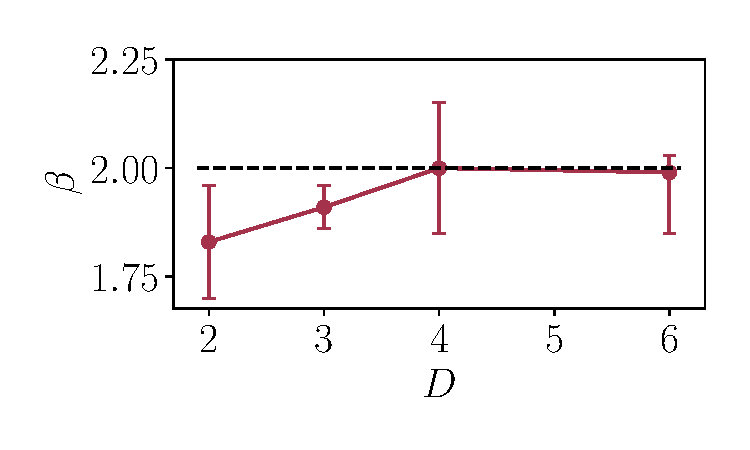
\includegraphics[width=0.5\textwidth]{Chapitre3/Figures/Interpretation/D_dependence.pdf}
	\caption{Évolution de l'exposant critique $\beta$ en fonction de la dimension de l'espace $D$ dans le modèle $\alpha$-ROM avec sauts infinis des particules actives et $\alpha = 0$.}
	\label{fig:Ddep}
\end{figure}

\subparagraph{}Ainsi, dans la limite de grande dimension où la dynamique des particules passives est simplifiée, nous mesurons effectivement $\beta \approx 2$. Cela suggère que l'image proposée par le modèle $\mu$-Hébraud-Lequeux est effectivement adéquate pour décrire le mécanisme de diffusion des particules passives dans le $\alpha$-ROM dans la limite champ moyen.

\paragraph{Interprétation champ moyen du mécanisme de diffusion en dimension finie}

\subparagraph{}En pratique, les systèmes réels d'intérêt ne se situent pas exactement dans les limites de champ moyen. Toutefois, nous pouvons parfois espérer que le cadre champ moyen associé puisse être capable de rendre compte de certains aspects hors de ces limites. Dans cette optique, nous proposons d'étudier le modèle défini précédemment (i.e. avec sauts infinis des particules actives) en 2D, dimension d'intérêt pour ce travail, et pour différentes portées d'interaction $\alpha$. Dans cette version du $\alpha$-ROM, les sauts infinis des particules actives permettent de laisser le contrôle de la criticalité au mécanisme de diffusion, mais dans une limite non-triviale de basse dimension que l'on retrouve dans le $\alpha$-ROM original. Via ces sauts infinis, nous nous attendons à une validité de la relation $\mu = D/\alpha$ en raison de la décorrélation des positions des particules actives. Toutefois, la dynamique des particules passives prenant place dans un espace de dimension finie, il est probable que les relations entre les exposants $\mu$, $\theta$ et $\beta$ se voient modifiées. 

\subparagraph{}Pour comprendre ce qu'il subsiste de l'image champ moyen à cette dimension, nous nous concentrons dans ce cas sur les portées $\alpha \in \{ 0.5, 1, 1.25, 1.5, 2, 2.5, 3 \}$, et nous nous intéressons aux exposants $\beta$ puis $\theta$ associés.

\paragraph{Évolution de la convexité}

\label{sec:sautsinfinis}

\subparagraph{}Pour déterminer l'évolution de la convexité dans ce modèle simplifié, nous menons la même analyse que dans le cas du $\alpha$-ROM à la \autoref{sec:TBLRRStat}. Sur la \autoref{fig:mueff}-(a), nous représentons l'évolution de $\beta$ avec l'exposant de portée d'interaction $\alpha$ et, en pointillés noirs, le comportement champ moyen du modèle $\mu$-Hébraud-Lequeux pour $\mu = D/\alpha$. Malgré la dynamique a priori non-triviale des particules passives dans le modèle numérique, les deux évolutions présentent un très bon accord aux courtes portées $\alpha \gtrsim 1.5$. Plus particulièrement, comme l'image champ moyen le prédit, l'influence du bruit interne sur la criticalité prend place à partir de $\alpha = D = 2$. De manière remarquable, le modèle $\mu$-Hébraud-Lequeux semble donc permettre de rationaliser partiellement la zone continue d'évolution de la criticalité dans ce modèle 2D.

\subparagraph{}Pour les plus grandes portées $\alpha\lesssim 1.5$, si un accord qualitatif est remarqué, le modèle en dimension finie se démarque de l'image champ moyen comme nous le pensions du fait de la dynamique réelle des particules passives.

\begin{figure}[h]
	\centering
	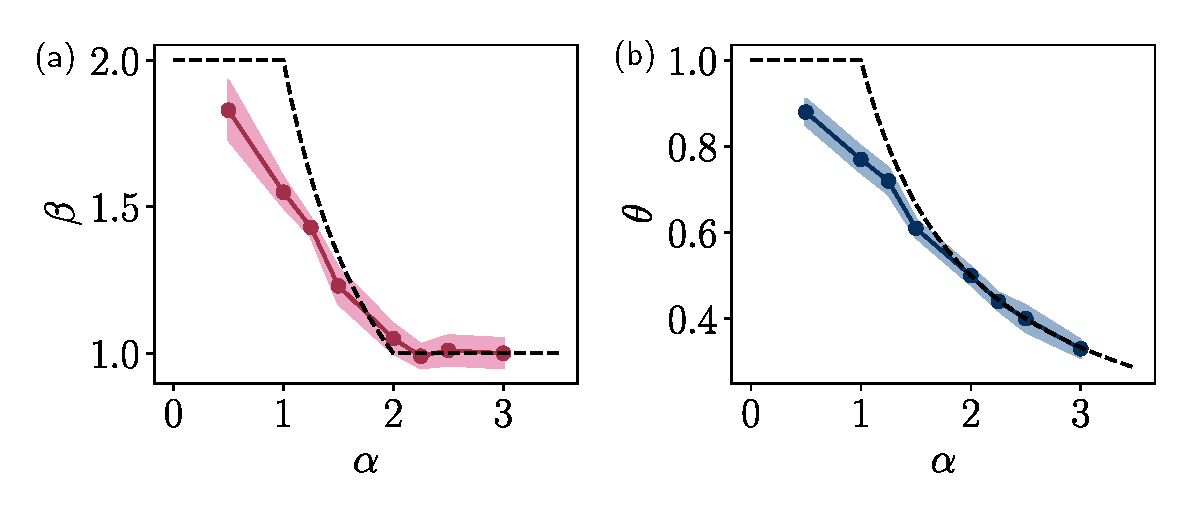
\includegraphics[width=0.8\textwidth]{Chapitre3/Figures/Interpretation/beta_alphaMF.pdf}
	\caption{(a) Évolution de l'exposant $\beta$ avec la portée des interactions $\alpha$ dans le $\alpha$-ROM en 2D avec sauts infinis des particules actives. (b) Idem mais pour l'exposant de pseudo-gap $\theta$. Dans les deux cas, les pointillés noirs représentent les prédictions du modèle $\mu$-Hébraud-Lequeux avec $\mu = D/\alpha$.}
	\label{fig:mueff}
\end{figure}

\paragraph{Évolution de la distribution des distances à l'activation}

\subparagraph{}Pour tester la pertinence de l'image champ moyen concernant l'exposant $\theta$ dans un cadre de dimension finie, nous proposons tout d'abord une manière de le déterminer dans les modèles numériques dérivés du ROM. Dans le cadre de ces modèles, la distance à l'activation d'une particule peut être associée à la distance à la particule voisine la plus proche. Sous cet angle, la fonction de corrélation de paire entre particules passives $g^p(r)$ semble être l'objet physique le plus adéquat pour caractériser cette propriété. Plus précisément, étant donné que $g^p(r<D_p)=0$ dû à la condition de recouvrement, nous nous attendons à ce que la fonction $g(x) = g^p(r-D_p)$ se comporte comme la distribution $P(R-|\mathbf{r}|)$ du modèle $\mu$-Hébraud-Lequeux. Bien que la fonction de corrélation de paire ne représente pas directement une probabilité de présence du plus proche voisin, nous nous attendons à ce que ce soit le cas asymptotiquement à petits $x$. Ainsi, nous nous attendons, dans le cas idéal où l'image champ moyen est parfaitement retrouvée, à mesurer dans nos simulations numériques au point critique :

\begin{equation}
	g(x) \sim x^\theta, \quad \theta = \left\{
	\begin{aligned}
	&\frac{\mu}{2}, \quad \mu \leq 2\\
	&1, \quad \mu \geq 2
	\end{aligned}
	\right.
	\label{eq:gpass}
\end{equation}

\subparagraph{}Nous proposons alors d'évaluer cet exposant $\theta$ dans le $\alpha$-ROM en 2D avec sauts infinis des particules actives. Nous mesurons donc la fonction de corrélation de paire entre particules passives $g^p(r)$ à petits $r$, pour différentes distances au point critique $\delta\phi$ et ce pour chaque portée $\alpha$. Un exemple de mesures pour $\alpha = 1.5$ et $\alpha = 5$ est présenté sur les encarts de la \autoref{fig:PCorr_alphaMF}. Une première chose remarquable est que, même si nous considérons un cas de dimension finie ici, nous observons effectivement un comportement algébrique de $g(x)$ avec $x$ qui s'étend à petits $x$ à mesure que le point critique est approché. La prédiction du modèle champ moyen $\mu$-Hébraud-Lequeux quant à une distribution algébrique des distances à l'activation semble donc retrouvée dans ce modèle.

\subparagraph{}\`A très petits $x$, la fonction de corrélation sature sur un plateau dont la valeur décroît avec la distance au point critique. Cela s'explique probablement par le fait que le comportement donné par l'\autoref{eq:gpass} n'est en fait valable qu'au point critique, comme c'est le cas dans le modèle $\mu$-Hébraud-Lequeux. De ce fait, la détermination directe de l'exposant $\theta$ est rendue difficile, puisque le régime de loi de puissance est parasité par ce plateau. Pour s'affranchir de cet effet, nous utilisons une méthode de redimensionnement par $\delta\phi$ pour mesurer l'exposant $\theta$. Cette méthode est alors très similaire à celle présentée à la \autoref{sec:expdynjump} pour la détermination de l'exposant $\delta$. Pour ce faire, nous supposons donc que la fonction $g^p(x=r-D_p, \delta\phi)$ est homogène de ses arguments dans le régime critique. Dans le cadre de cette hypothèse, en redimensionnant $g^p(x, \delta\phi)$ par $\delta\phi^{a_1}$ et $x$ par $\delta\phi^{a_2}$, il est possible de trouver $a_1$ et $a_2$ tels que les courbes pour différents $\delta\phi$ se superposent toutes sur une courbe maîtresse. Si cette superposition est effectivement réalisable, l'exposant $\theta$ caractérisant le comportement de la fonction avec $x$ est alors directement donné par $\theta = a_1/a_2$.

\begin{figure}[h]
	\centering
	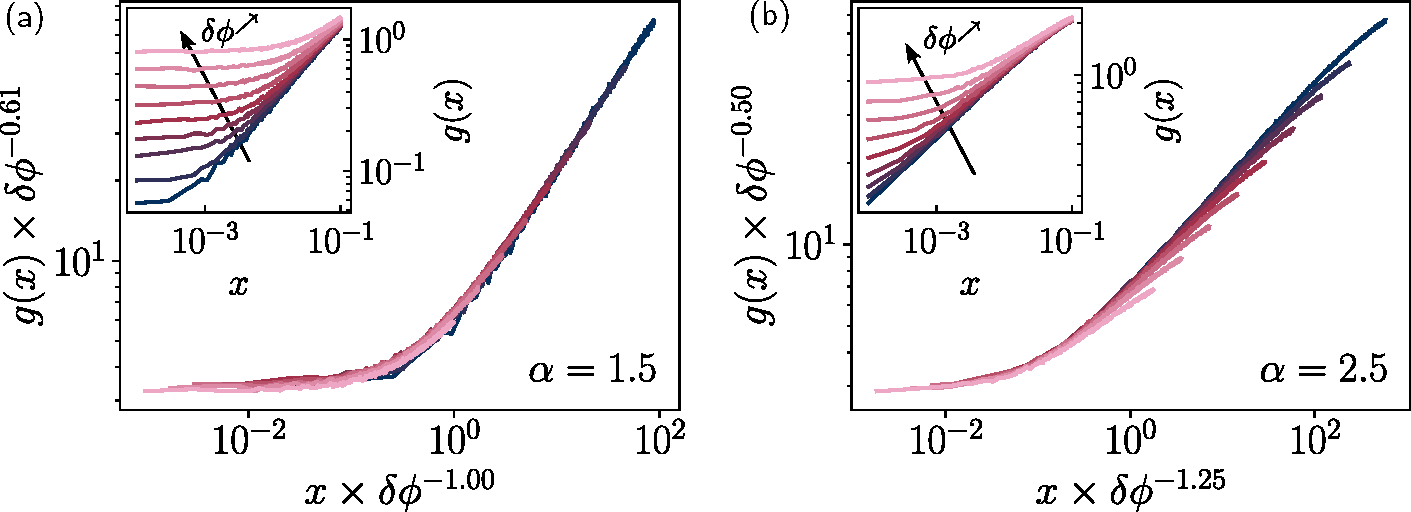
\includegraphics[width=\textwidth]{Chapitre3/Figures/Interpretation/PCorr_alphaMF.pdf}
	\caption{Redimensionnement des fonctions de corrélation de paire entre particules passives avec la distance au point critique $\delta\phi$ dans le $\alpha$-ROM en 2D avec sauts infinis des particules actives pour $\alpha = 1.5$ (a) et $\alpha=2.5$ (b). En encart, les données brutes associées.}
	\label{fig:PCorr_alphaMF}
\end{figure}

\subparagraph{}Nous représentons à la \autoref{fig:PCorr_alphaMF} le meilleur redimensionnement par $\delta\phi$ obtenu dans les cas $\alpha = 1.5$ et $\alpha=5$ et reportons le cas des autres portées dans l'\annexeref{sec:PCorr}. Comme on peut le remarquer, la superposition des courbes est remarquablement satisfaisante sous le bon choix d'exposants. Notre hypothèse d'homogénéité de la fonction $g^p(x, \delta\phi)$, que nous notons plus simplement $g(x)$ laissant la dépendance en $\delta\phi$ implicite, est donc bien validée. Une information annexe que nous tirons de ces redimensionnements est que, pour $\theta>0.5$, nous mesurons $a_1 = \beta/2$ ce qui signifie que la valeur au contact $x=0$ de la fonction $g$ évolue comme $\delta\phi^{\beta/2}$. De plus, pour $\theta<0.5$, là où nous avons mesuré $\beta=1$, celle-ci évolue comme $\delta\phi^{0.5}$. Ainsi, par définition de l'exposant $\beta$ ($\langle A \rangle \sim \delta\phi^\beta$), la valeur du plateau se comporte comme $\sqrt{\langle A \rangle}$ à toute portée. La forme adéquate de la fonction de corrélation de paire à une distance finie du point critique est donc :

\begin{equation}
	g(x) \sim \sqrt{\langle A \rangle} + x^\theta
	\label{eq:scalinggx}
\end{equation}

\subparagraph{}Pour en revenir à la mesure de l'exposant $\theta$ et son évolution avec la portée, nous traçons sur la \autoref{fig:mueff}-(b) l'évolution de l'exposant $\theta$ mesuré par redimensionnement avec $\alpha$ et, en pointillés noirs, le comportement du modèle $\mu$-Hébraud-Lequeux pour $\mu = D / \alpha$. De manière similaire à l'étude de la convexité, nous remarquons un comportement quantitativement comparable entre le modèle numérique et l'image champ moyen à courte portée $\alpha \gtrsim 1.5$. \`A plus longue portée, nous retrouvons de nouveau un écart avec l'image champ moyen.

\paragraph{Complexité dans la dynamique des particules passives}

\subparagraph{}De manière remarquable, certaines prédictions du modèle champ moyen semblent être vérifiées dans le $\alpha$-ROM avec sauts infinis des particules actives en dimension finie. Notamment, nous retrouvons un impact du mécanisme de diffusion sur la criticalité à partir de $\alpha = D = 2$ et un accord quantitatif sur les courbes $\beta(\alpha)$ et $\theta(\alpha)$ à courte portée. Dans cette partie nous montrons que même si les relations $\beta(\alpha)$ et $\theta(\alpha)$ ne sont plus champ moyen à longue portée, une loi d'échelle du modèle $\mu$-Hébraud-Lequeux reste toujours vérifiée dans ce cas.

\subparagraph{}Les relations $\beta(\alpha)$ et $\theta(\alpha)$ dans le modèle $\mu$-Hébraud-Lequeux sont en fait une combinaison de résultats issus de différentes hypothèses. Elles se basent sur la relation entre $\mu$ et $\alpha$, celle entre $\theta$ et $\mu$, puis celle entre $\beta$ et $\theta$ et $\mu$ \cite{lin_microscopic_2018}. Une manière de tester la pertinence de l'image champ moyen en dimension finie peut être de se concentrer sur une de ces sous-relations, par exemple, la relation d'échelle $\beta = 2\theta$. Sur la \autoref{fig:2thetaMF}, nous superposons donc les évolutions de $2\theta$ et $\beta$ dans le cas du $\alpha$-ROM avec sauts infinis des particules actives. 

\subparagraph{}De manière remarquable, nous observons que la loi d'échelle $\beta = 2\theta$ pour $\theta > 0.5$ est vérifiée à toutes les portées, même à petit $\alpha$, où l'on n'observe plus $\beta=D/\alpha$ ou $2\theta=D/\alpha$. Ainsi, il semblerait que même dans le domaine où la dynamique des particules passives en dimension finie écarte le modèle numérique de l'image champ moyen, nous retrouvons un lien direct entre la convexité de la transition et la forme de la fonction de corrélation de paire. En ce sens, le modèle $\mu$-Hébraud-Lequeux reste un cadre intéressant pour analyser le mécanisme de diffusion même en dimension finie. Cette observation confirme les résultats préliminaires de la sous-sous-section précédente, plaçant effectivement le modèle $\mu$-Hébraud-Lequeux comme le cadre de description adéquat du mécanisme de diffusion.

\begin{figure}[h]
	\centering
	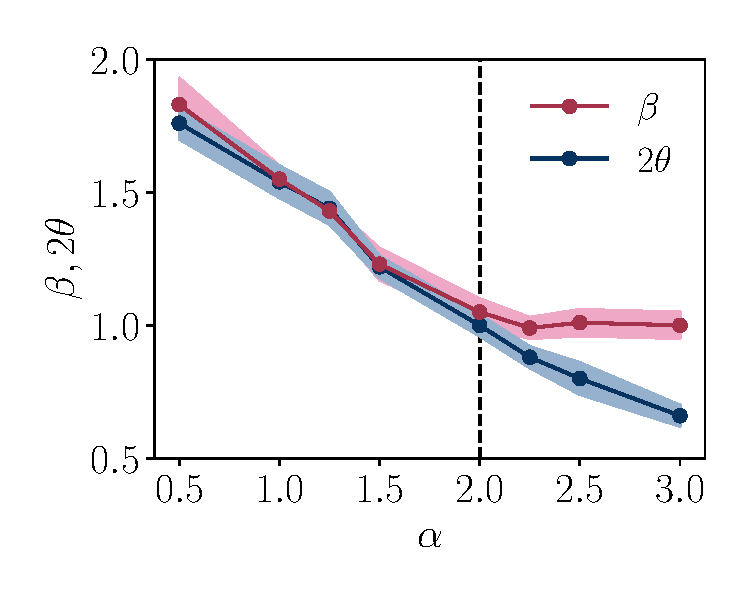
\includegraphics[width=0.5\textwidth]{Chapitre3/Figures/Interpretation/beta_theta_alphaMF.pdf}
	\caption{Comparaison de l'évolution des exposants $\beta$ et $\theta$ avec la portée $\alpha$ dans le cadre du $\alpha$-ROM en 2D avec sauts infinis des particules actives. La ligne pointillée noire représente $\alpha = 2$ soit $\mu=1$ dans le modèle $\mu$-Hébraud-Lequeux avec $\mu=D/\alpha$.}
	\label{fig:2thetaMF}
\end{figure}


\subsubsection{Image champ moyen dans le $\alpha$-ROM}

\subparagraph{}Dans le cadre du $\alpha$-ROM avec sauts finis des particules actives, pour les raisons que nous avons évoquées précédemment, nous ne nous attendons pas à ce que les prédictions de l'image champ moyen puissent se retrouver dans l'analyse du modèle numérique. Toutefois, comme nous le montrons dans cette sous-sous-section, une comparaison avec le modèle $\mu$-Hébraud-Lequeux et avec le modèle numérique avec sauts infinis des particules actives peut amener à des observations intéressantes.

\paragraph{Évolution de la convexité : une influence moindre des corrélations d'activité ?}

\subparagraph{}Sur la \autoref{fig:BetaMu1}-(a), nous comparons les évolutions de l'exposant $\beta$ avec $\alpha$ pour le $\alpha$-ROM en 2D et en 3D avec les prédictions du modèle $\mu$-Hébraud-Lequeux pour $\mu = D/\alpha$. De manière attendue, nous n'observons d'accord quantitatif dans aucune limite : les mesures numériques présentent systématiquement une convexité moindre. Dans la limite de courte portée, ce désaccord est évident. En effet, dans ce cas-là la criticalité est celle de la classe CDP, dominée par la dynamique des particules actives, et n'a donc rien à voir avec le mécanisme proposé par l'image champ moyen. Nous notons toutefois qu'étant donné que l'exposant $\beta_\text{CDP}$ augmente avec la dimension pour arriver à $\beta = 1$ pour $D=4$, en augmentant la dimension, l'écart observable se réduit entre les points de mesure et les pointillés dans la limite gauche du graphique.

\begin{figure}[h]
	\centering
	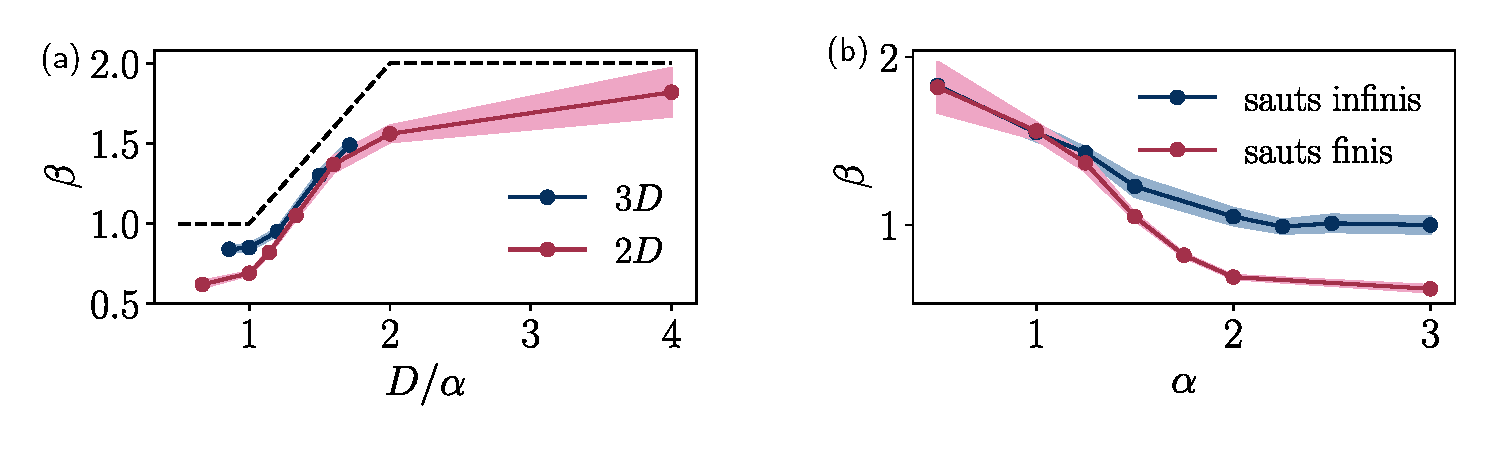
\includegraphics[width = \textwidth]{Chapitre3/Figures/Interpretation/Beta_Mu1.pdf}
	\caption{(a) Évolution de l'exposant $\beta$ en fonction de $D/\alpha$ dans le $\alpha$-ROM en 2D et en 3D. En pointillés noirs, nous représentons les prédictions du modèle $\mu$-Hébraud-Lequeux avec $\mu = D/\alpha$. (b) Comparaison de l'évolution de l'exposant $\beta$ avec $\alpha$ dans le cas du $\alpha$-ROM et du $\alpha$-ROM avec sauts infinis des particules actives en 2D.}
	\label{fig:BetaMu1}
\end{figure}

\subparagraph{}Dans la limite de longue portée, cet écart n'est pas non plus surprenant puisque dans la partie précédente concernant le modèle avec sauts infinis des particules actives, nous l'avons attribué à la dynamique des particules passives, qui reste intacte dans le cas du $\alpha$-ROM. Toutefois, nous pouvons noter quelque chose de plus intéressant dans cette zone. Sur la \autoref{fig:BetaMu1}-(b), nous comparons les résultats obtenus en 2D dans le cas de sauts finis et de sauts infinis des particules actives (resp. activité corrélée et activité décorrélée). Comme nous pouvons le remarquer, à longue portée $\alpha \lesssim 1.25$ les résultats associés aux deux modèles convergent. Cela suggère alors que la dynamique de l'activité n'influence pas, via la modification de la relation $\mu=D/\alpha$ ou via le mécanisme additionnel de création de l'activité par transport des particules actives, le comportement critique dans cette limite. Ainsi, à longue portée, la création d'activité dans le $\alpha$-ROM semble être dominée par le mécanisme de diffusion induit non-localement par l'activité (voir \autoref{eq:meca_diff}).

\subparagraph{}Une observation remarquable par ailleurs est que dans le cas $2D$ et $3D$, l'influence des interactions à longue portée sur la criticalité débute en $\alpha = D$, comme le prédit le modèle $\mu$-Hébraud-Lequeux avec $\mu = D/\alpha$, et comme cela a été mesuré dans le cas du modèle avec sauts infinis. 

\paragraph{Évolution de l'exposant $\theta$ de pseudo-gap}

\subparagraph{}Dans la dynamique complexe offerte par le $\alpha$-ROM, dû à la dynamique annexe des particules actives, il n'est pas évident que la fonction de corrélation de paire présente un comportement algébrique comme dans les modèles isolant le mécanisme de diffusion. Pour le vérifier, nous effectuons les mêmes mesures de fonctions de corrélation de paire que dans la partie précédente pour le $\alpha$-ROM en 2D (avec sauts finis des particules actives donc). Simplement, du fait des résultats de l'analyse précédente, nous choisissons de redimensionner directement les quantités par $\langle A \rangle$ et non $\delta\phi$ (voir l'\autoref{eq:scalinggx}). Les redimensionnements les plus convaincants obtenus sont alors représentés pour $\alpha=0.5$ et $\alpha=1.25$ à la \autoref{fig:PCorr_alpha}. Les autres analyses sont reléguées dans l'\annexeref{sec:PCorr}. 

\begin{figure}[h]
	\centering
	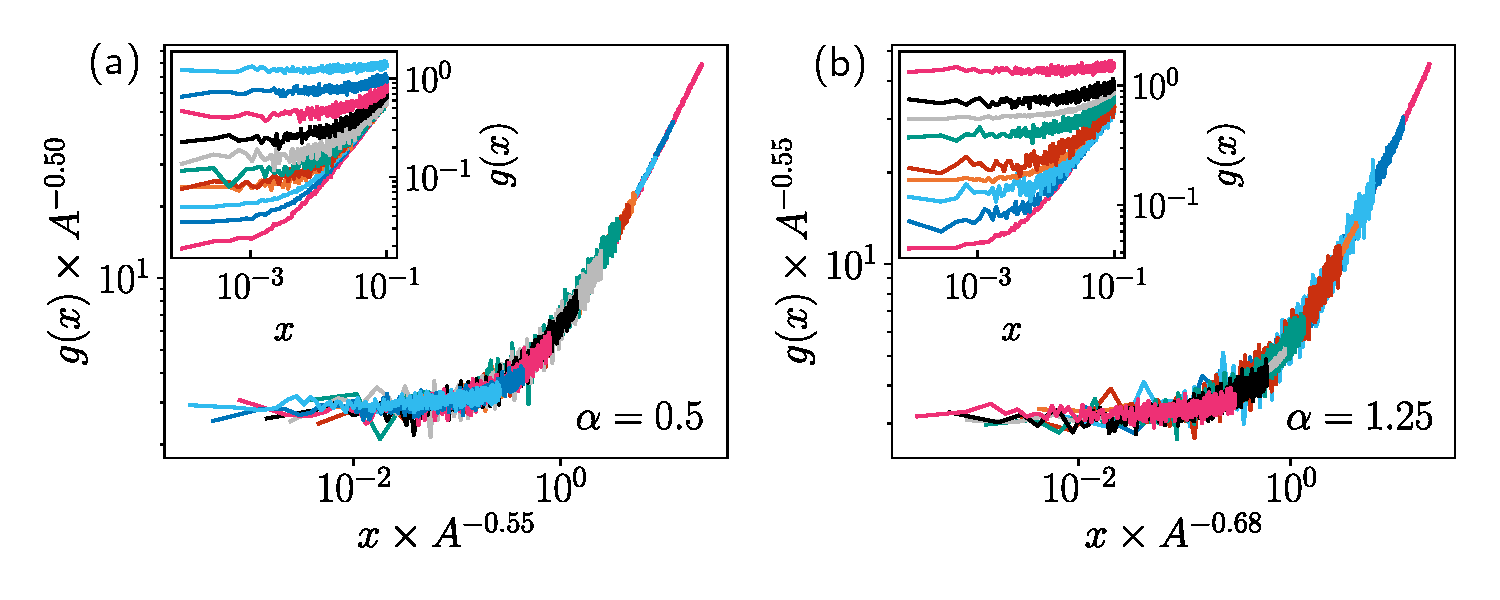
\includegraphics[width=\textwidth]{Chapitre3/Figures/Interpretation/PCorr_alpha.pdf}
	\caption{Redimensionnement des fonctions de corrélation de paire entre particules passives avec l'activité moyenne $\langle A \rangle$ dans le $\alpha$-ROM en 2D avec sauts finis des particules actives pour $\alpha = 0.5$ (a) et $\alpha=1.25$ (b). En encart, les données brutes associées.}
	\label{fig:PCorr_alpha}
\end{figure}

\subparagraph{}La superposition des courbes est alors toujours satisfaisante, même si un peu moins nette, pour tout $\alpha$. Cela montre que même en présence de la dynamique corrélée des particules actives, les fonctions de corrélation de paire possèdent un caractère non-trivial, signe de la présence du mécanisme de diffusion capturé par l'image champ moyen. Dans le cas de très longue portée, nous retrouvons un comportement en $\sqrt{\langle A \rangle}$ de $g(0)$. Toutefois ce comportement semble perdu à plus courtes portées où l'on mesure $g(0)\sim A^b$ avec $b>0.5$ dès $\alpha = 1$. Nous sommes finalement capables d'extraire des valeurs de $\theta$ pour chaque $\alpha$. Sur la \autoref{fig:Beta_Theta}, nous représentons l'évolution de $2\theta$ avec $\alpha$ et la mettons en regard de l'évolution de l'exposant $\beta$ mesurée à la \autoref{sec:TBLRRStat}.

\begin{figure}[h]
	\centering
	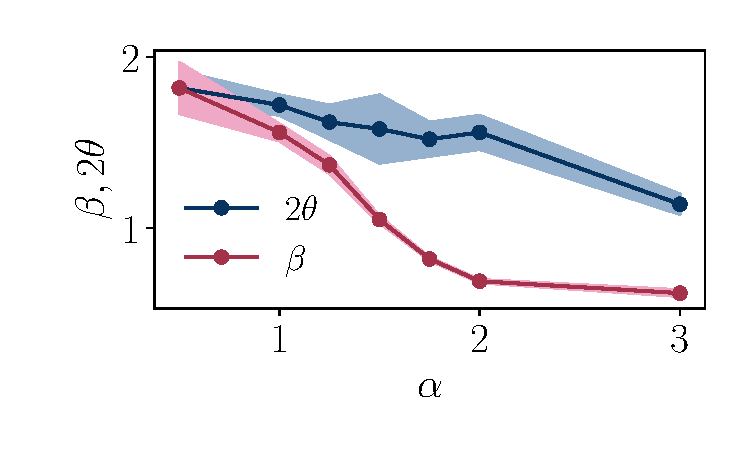
\includegraphics[width=0.6\textwidth]{Chapitre3/Figures/Interpretation/Beta_Theta.pdf}
	\caption{Comparaison de l'évolution de $\beta$ et $2\theta$ avec $\alpha$ dans le cas du $\alpha$-ROM en 2D.}
	\label{fig:Beta_Theta}
\end{figure}

\subparagraph{}Nous observons alors une évolution de l'exposant $\theta$ qualitativement en accord avec l'image champ moyen, soit une tendance d'augmentation avec la portée des interactions. Celle-ci semble cependant différente de celle observée dans le cas du modèle à sauts infinis. En effet, l'évolution observée ici est d'une amplitude moindre et nous n'observons par exemple pas de tendance réellement significative dans la zone $1.5 \leq \alpha \leq 2$, là où l'exposant $\beta$ varie pourtant fortement.

\subparagraph{}Si l'on compare les évolutions de $2\theta$ et $\beta$ nous remarquons des divergences claires, signifiant que la relation d'échelle $2\theta = \beta$ n'est plus vérifiée pour tout $\theta > 0.5$. Cette observation est attendue, puisque l'image champ moyen ne permet de toute façon pas de rendre compte d'un exposant $\beta < 1$, ce que l'on a mesuré pour $\alpha \gtrsim 1.5$. Toutefois, de manière remarquable, l'écart entre ces deux quantités ($\beta$ et $2\theta$) se réduit à mesure que la portée augmente, si bien que dans la limite de très grande portée $\alpha = 0.5$ l'accord est retrouvé. Cela conforte l'idée selon laquelle à grande portée, la dynamique de l'activité n'influence plus significativement le comportement critique.

\subsubsection{Conclusion de la sous-section}

\subparagraph{}En conclusion, cette sous-section nous a permis de tester la pertinence de l'image champ moyen pour comprendre le mécanisme de diffusion des particules passives et son influence dans les modèles numériques étudiés. Via l'étude d'une version simplifiée du $\alpha$-ROM, nous avons montré que le modèle $\mu$-Hébraud-Lequeux permet effectivement de rationaliser l'effet du mécanisme de diffusion sur la criticalité malgré la présence d'une dynamique non-triviale des particules passives. 

\subparagraph{}Dans le cas d'une dynamique plus complexe représentée par le modèle $\alpha$-ROM, les prédictions du modèle champ moyen ne tiennent plus de manière générale mais nous permettent de retrouver des traces de l'influence de la diffusion des particules passives. Notamment, nous remarquons une forme algébrique de la fonction de corrélation de paire proche du contact, décrite par un exposant de pseudo-gap $\theta$. De manière remarquable, nous observons par ailleurs que dans la limite de grande portée, la dynamique d'activité dans le modèle ne semble plus contrôler la convexité de la transition, faisant du modèle $\mu$-Hébraud-Lequeux le champ moyen adéquat pour appréhender la dynamique complète.

\subsection{Disqualification complète du cadre LR-CDP}

\subparagraph{}Les analyses précédentes nous ont permis de montrer en quoi la diffusion des particules passives induite non-localement par l'activité représentait un mécanisme essentiel dans la transition du $\alpha$-ROM. Toutefois, à courte portée au minimum, il ne semble pas que celle-ci suffise à comprendre entièrement la criticalité du modèle. Notamment, les cas où l'on mesure $\beta < 1$ ne peuvent être compris sans les corrélations induites par les sauts des particules actives et le mécanisme de création de l'activité qu'elles représentent. Bien que la zone $\beta >1$ soit hors d'atteinte du cadre de référence LR-CDP, il est tentant de vouloir interpréter cette zone $\beta < 1$ via ce formalisme. Dans ce scénario, le paysage global présenté à la \autoref{sec:TBLRRStat} se formerait donc d'une zone convexe avec $\beta>1$ dominée par la dynamique des particules passives, et d'une zone concave avec $\beta<1$ interprétable comme une zone dominée par la dynamique des particules actives.

\subparagraph{}Un premier conflit d'interprétation de cette région concave par ce scénario vient du fait que la zone d'exposants $\alpha$ pour laquelle on passe de $\beta\approx 0.64$ en 2D à $\beta=1$ n'est pas du tout la même que celle du cadre LR-CDP. En effet, nous avons identifié $1.5\lesssim \alpha \lesssim 2$ pour le $\alpha$-ROM et $3<\alpha<4$ pour LR-CDP en 2D. Toutefois, nous pourrions imaginer que le mécanisme de diffusion dans cette zone agisse de la même manière qu'un transport à longue portée, seulement avec un exposant effectif de transport différent. Il serait alors possible de rattacher le $\alpha$-ROM au cadre d'interprétation de l'influence d'un transport à longue portée dans cette zone concave. 

\subparagraph{}Dans le cas d'un transport à longue portée contrôlé par l'exposant $\gamma$, une particule active dans un espace de dimension $D$ fait un saut dont l'amplitude $\Delta$ suit une distribution $P(\Delta)\sim\Delta^{D-1-\gamma}$ (voir \autoref{chapter:TransportLP}). En supposant la densité de particules homogène dans le système, cela correspond pour la particule active à une probabilité $P_a(r)$ de créer de l'activité à une distance $r$ à l’issue du pas de temps telle que :

\begin{equation}
	P_a(r) \sim \frac{1}{r^{1+\gamma-D}}
	\label{eq:sautabsoupas}
\end{equation}

\noindent La question est alors de savoir si une telle quantité peut être dérivée dans le cas du $\alpha$-ROM, et comment celle-ci se compare au cas du transport à longue portée à comportement critique équivalent. En d'autres termes, peut-on dériver un exposant de saut effectif $\gamma_\text{eff}$ dans le cadre de ce modèle ? 

\subparagraph{}Pour ce faire, nous considérons la portée $\alpha = 1.75$ pour laquelle nous avions mesuré $\beta\approx 0.82$ dans le $\alpha$-ROM en 2D. Elle se situe donc à mi-chemin entre la limite de courte portée $\beta = 0.64$ et la valeur triviale $\beta = 1$, et donc cette criticalité peut-être atteinte dans le cadre du transport à longue portée. Pour ce faire, nous générons un état absorbant du système à $\phi = \phi_c$. \`A partir de cet état absorbant, nous activons aléatoirement une particule, générant alors un saut de courte portée et un bruit sur toutes les autres particules passives. En identifiant les particules activées suite à ce pas de temps et leur distance $r$ à la particule activée, nous pouvons mesurer la quantité $P_a(r)$ dans ce cadre. Le même protocole peut être appliqué dans le cadre du transport à longue portée (en faisant usage du LR-ROM). Pour un système de taille $L=4096$, nous comparons alors la mesure de $P_a(r)$ obtenue pour $\alpha = 1.75$ à celle obtenue dans le cas d'un transport à longue portée avec $\gamma = 3.5$. La valeur de $\gamma$ est choisie ainsi puisque dans ce cas nous avions mesuré $\beta \approx 0.81$ (voir \autoref{sec:expcritjumps}), soit une valeur très proche de $\beta\approx 0.82$ pour $\alpha = 1.75$ dans le cas du $\alpha$-ROM. Les résultats obtenus sont présentés sur la \autoref{fig:RangeInterpretation}.

\begin{figure}[h]
	\centering
	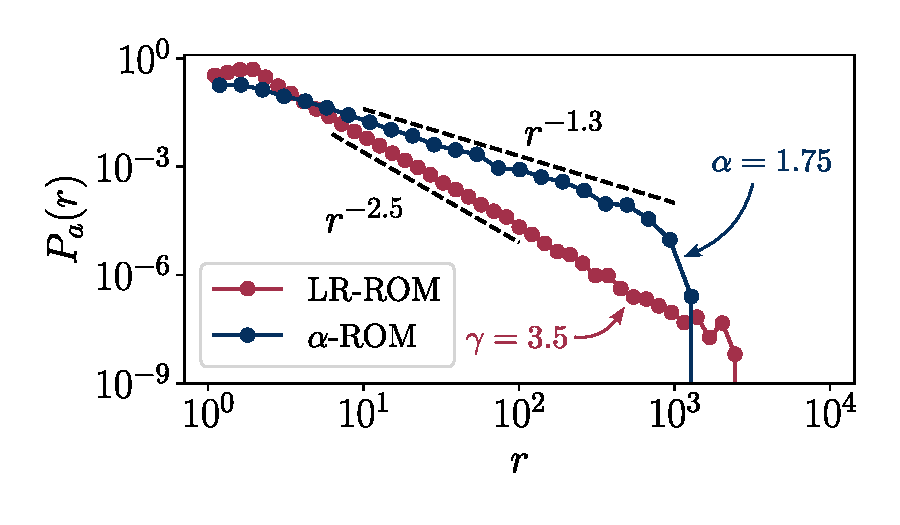
\includegraphics[width=0.65\textwidth]{Chapitre3/Figures/Interpretation/RangeInterpretation.pdf}
	\caption{Évolution des distributions $P_a(r)$ pour le LR-ROM avec $\gamma = 3.5$ et pour le $\alpha$-ROM avec $\alpha = 1.75$.}
	\label{fig:RangeInterpretation}
\end{figure}

\subparagraph{}Nous constatons alors que dans le cas du transport à longue portée, $P_a(r)$ décroît bien comme $1/r^{2.5}$ soit $\gamma - 1$ en 2D (voir l'\autoref{eq:sautabsoupas}). Dans le cas du $\alpha$-ROM, cette distribution décroît comme $1/r^{1.3}$ soit $\gamma_\text{eff}\approx 2.3$, donc bien moins rapidement. En réalisant ces mêmes mesures sur des états actifs de la dynamique, les mêmes observations peuvent être faites. Ainsi, si les deux modèles partagent le même exposant $\beta$ à ces portées, ils ne partagent pas du tout les mêmes propriétés de création d'activité. En d'autres termes, il ne semble pas possible d'interpréter la criticalité du $\alpha$-ROM via le cadre LR-CDP, même dans la zone concave $\beta < 1$. La dynamique des particules passives reste donc importante à toute portée $\alpha < D$ et le changement de convexité ne semble pas relever d'un changement abrupt de mécanisme prépondérant.

\subsection{Conclusion de la section}

\subparagraph{}En conclusion, nous avons établi dans cette section un modèle de type champ moyen permettant une transition de réversibilité convexe. Son étude révèle alors la place essentielle du bruit interne, i.e. de la diffusion des particules passives induite non-localement par l'activité, dans la criticalité du $\alpha$-ROM. Notamment, dans la limite de très longue portée $\alpha\rightarrow 0$, ce mécanisme de création de l'activité semble pouvoir décrire à lui seul la transition. Enfin, si la zone concave pour laquelle on retrouve $\beta<1$ prend l'apparence du comportement attendu dans le cadre LR-CDP, celle-ci correspond en fait à une dynamique bien différente. In fine, via la présence supplémentaire du mécanisme de diffusion des particules, le modèle $\alpha$-ROM est donc différent en tout point du cadre LR-CDP sous les aspects abordés et nécessite un traitement théorique fondamentalement différent.

\section{Avalanches}

\subparagraph{}Afin de souligner ces différences par un dernier aspect incontournable de la criticalité absorbante, nous proposons d'étudier dans cette section la dynamique d'avalanche à l’œuvre dans le $\alpha$-ROM.

\label{sec:AvSusp}

\subsection{Avalanches à densité fixée}

\subsubsection{Redéfinition}

\subparagraph{}Comme nous l'avons vu au \autoref{chapter:introduction}, les modèles appartenant à la classe CDP présentent une dynamique d'avalanche. Pour la mettre en évidence, il est d'usage de se placer dans le cadre de la criticalité auto-organisée (abrégée SOC pour \textit{self-organized criticality}). Dans celui-ci, la séparation d'échelle entre le temps de forçage (ajout de matière aléatoire) et de relaxation (disparition de matière induite par l'activité) permet d'observer distinctement des évènements d'activité fortement corrélés et distribués de manière algébrique : ce sont les avalanches.

\subparagraph{}Une autre manière d'observer la dynamique critique est de se placer dans l'état stationnaire à une densité fixée de particules $\phi$ dans le système, proche de la densité critique $\phi_c$. Le fait est que, dans ces conditions, le système est proche d'une transition de phase absorbante. Ainsi, pour un système de taille finie, du fait des fluctuations de la dynamique, cette dernière peut régulièrement tomber dans un état absorbant pour $\phi \gtrsim \phi_c$. Pour sonder la dynamique d'avalanche à densité imposée, il est donc nécessaire de réactiver le système à chaque fois qu'il se retrouve bloqué. Un protocole généralement utilisé est alors d'activer artificiellement une particule dans le système, précurseur de l'évènement \cite{lubeck_universal_2003, vespignani_absorbing_state_2000, munoz_avalanche_1999}.

\subparagraph{}Cette situation impose de redéfinir la notion d'avalanches à densité fixée. Dans ce cadre, nous définissons une avalanche comme l'évènement ayant lieu entre deux réactivations du système. Il est alors possible de définir ces évènements exactement de la même manière que les avalanches dans le cadre de la SOC, i.e. par leur taille $S$, leur durée $T$ et le nombre de particules $N$ qu'ils impliquent. Dans le cadre du $\alpha$-ROM, la taille d'une avalanche correspond au nombre d'évènements d'activité individuels ayant lieu pendant l'évènement global. La durée correspond alors simplement au nombre de pas de temps entre le début et la fin de l'avalanche. Plusieurs études ont montré que ces avalanches étaient de même nature que celles du cadre de la SOC dans les modèles à courte portée\footnote{Ces études n'interprétaient cependant pas ces évènements à densité fixée comme des avalanches à proprement parler.} \cite{lubeck_universal_2003, vespignani_absorbing_state_2000, munoz_avalanche_1999}. Il est alors attendu que ces évènements soient aussi distribués de manière algébrique, définis par les exposants d'avalanche déjà présentés à la \autoref{sec:IntroAvalanches} :

\begin{equation}
	\begin{aligned}
		&P(S) \sim S^{-\tau}g_S\left( \frac{S}{S_c} \right), \quad S_c \sim L^{d_f}\\
		&P(T) \sim T^{-\tau^\prime}g_T\left( \frac{T}{T_c} \right), \quad T_c \sim L^{z}\\
		&P(N) \sim N^{-\tau^{\prime\prime}}g_N\left( \frac{N}{N_c} \right), \quad N_c \sim L^{\chi}\\
	\end{aligned}
	\label{eq:AvDistribSusp}
\end{equation}

\subparagraph{}Afin d'analyser le comportement des avalanches à la transition dans le cadre du $\alpha$-ROM, nous choisissons de nous placer à densité fixée. Ce choix se justifie par cohérence, les analyses précédentes ayant toutes été réalisées à densité fixée. Cela nous permet alors de caractériser directement la dynamique qui donne lieu au comportement critique précédemment déterminé.

\subsubsection{Protocole}

\subparagraph{}Pour étudier les avalanches à densité fixée dans le modèle $\alpha$-ROM, pour une portée $\alpha$ donnée, nous nous plaçons à la densité critique $\phi_c$ du système. Dès lors, nous générons un état absorbant du système en partant d'une configuration initiale aléatoire. \`A chaque fois que le système tombe dans un état absorbant, la dynamique est réactivée en activant artificiellement une particule choisie au hasard. Ce processus est alors réitéré suffisamment de fois pour obtenir une statistique propre et stationnaire pour les observables $S$, $T$ et $N$\footnote{En pratique, la stationnarité impose d'ignorer les premiers évènements.}. Nous réalisons alors ces mesures en 2D pour $\alpha \in \{ 3, 2, 1.75, 1.5, 1.25, 0.5\}$ et pour les tailles de systèmes $L \in \{ 256, 512, 1024, 2048 \}$. Un exemple des $3\times 4$ distributions\footnote{pour les trois grandeurs $S$, $T$ et $N$ et aux quatre tailles de systèmes.} obtenues est alors présenté à la \autoref{fig:AvSuspNotRescaled} pour $\alpha = 1.5$. Les mesures pour les autres portées $\alpha$ sont représentées dans l'\annexeref{sec:AvTBLRRAnnexe}.

\begin{figure}[h]
	\centering
	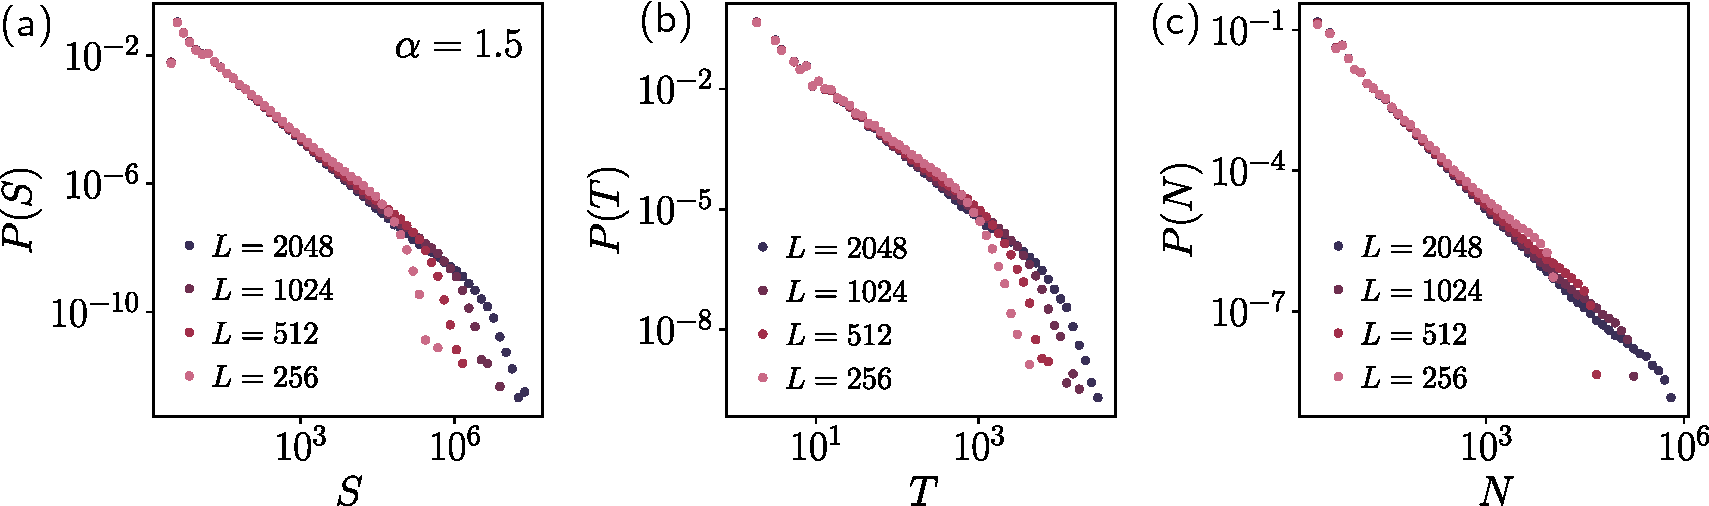
\includegraphics[width=\textwidth]{Chapitre3/Figures/Avalanches/Av_alpha15_edited.pdf}
	\caption{Distributions de taille (a), de durée (b) et du nombre de particules impliquées (c) pour les avalanches mesurées dans le modèle $\alpha$-ROM en 2D à densité fixée $\phi=\phi_c$ pour $\alpha = 1.5$ et pour $L \in \{ 256, 512, 1024, 2048 \}$.}
	\label{fig:AvSuspNotRescaled}
\end{figure}

\subparagraph{}Les formes des distributions sont alors celles supposées, présentant une décroissance en loi de puissance, commune à chaque taille, puis un cut-off, augmentant avec la taille du système. Par ailleurs, ce cut-off, dans le cas de $P(S)$ et $P(T)$, semble présenter une bosse qui s'étale à mesure que la portée augmente. Afin de déterminer précisément les exposants d'avalanche associés à ces distributions, nous procédons à une analyse d'échelle en taille finie. Pour ce faire, nous reprenons les formes définies par l'\autoref{eq:AvDistribSusp}. Selon ces ansatz, toute la dépendance des distributions en $L$ est portée par le cut-off. Prenons alors l'exemple de la distribution des tailles $P(S)$. En redimensionnant $S$ par $S_c$, nous obtenons :

\begin{equation}
	P(S) \sim L^{-d_f\tau}\tilde{S}^{-\tau}g_S\left( \tilde{S} \right),  \quad \tilde{S} = \frac{S}{L^{d_f}}
\end{equation}

\noindent Ainsi, en redimensionnant $P(S)$ par $L^{-d_f\tau}$ et $S$ par $L^{d_f}$, les courbes obtenues pour différentes tailles de systèmes $L$ sont indépendantes de $L$, i.e. se superposent. Ce principe constitue alors une méthode graphique de détermination des exposants : les exposants $d_f$ et $\tau$ sont déterminés comme ceux définissant le redimensionnement qui permet la meilleure superposition des courbes obtenues pour différents $L$. Nous représentons alors sur la \autoref{fig:AvSuspRescaled} la meilleure superposition obtenue pour $\alpha = 1.5$. Les représentations graphiques obtenues pour les autres portées sont reportées dans l'\annexeref{sec:AvTBLRRAnnexe} et les exposants ainsi déterminés sont tous reportés dans le \autoref{tab:expocritavsusp}.

\begin{figure}[h]
	\centering
	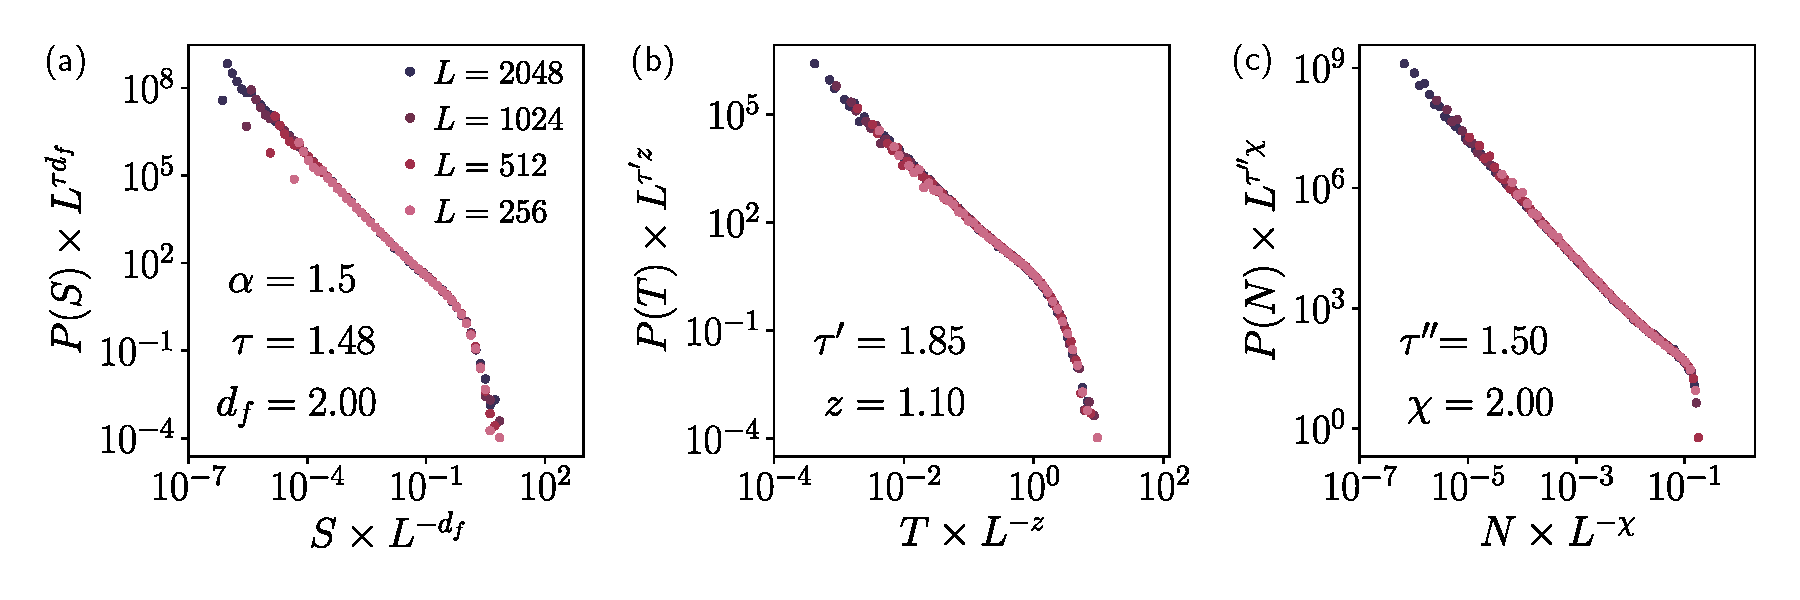
\includegraphics[width=\textwidth]{Chapitre3/Figures/Avalanches/Rescale_Av_alpha15.pdf}
	\caption{Redimensionnement par $L$ des distributions de taille (a), de durée (b) et du nombre de particules impliquées (c) pour les avalanches mesurées dans le modèle $\alpha$-ROM en 2D à densité fixée $\phi=\phi_c$ pour $\alpha = 1.5$ et pour $L \in \{ 256, 512, 1024, 2048 \}$.}
	\label{fig:AvSuspRescaled}
\end{figure}

\subsection{Évolution des exposants}

\subparagraph{}Pour les exposants $\tau$, $\tau^\prime$ et $\tau^{\prime\prime}$, nous observons une tendance d'augmentation avec la portée, comme dans le cadre LR-CDP/dépiégeage (voir \autoref{sec:LRCanonique}). Par exemple, on passe de $\tau\approx 1.28$ pour $\alpha=3$ à $\tau\approx 1.47$ pour $\alpha=1.25$. Nous remarquons par ailleurs que la valeur obtenue à courte portée $\alpha = 3$ est compatible avec les mesures déjà effectuées dans le cas de la classe CDP  \cite{chessa_critical_1999}. Nous notons cependant une anomalie à cette tendance d'augmentation pour $\alpha=0.5$, portée à laquelle le cut-off s'étale le plus sur la loi de puissance. Même si cette tendance générale est modérée, cela montre que les avalanches sont globalement distribuées de moins en moins largement à mesure que la portée des interactions augmente. De ce point de vue, l'évolution est alors similaire à celle du cadre LR-CDP, bien que la gamme de portées sur laquelle elle a lieu soit toujours très différente.

\subparagraph{}En revanche, les exposants de structure $d_f$, $z$ et $\chi$ sont soumis à des variations significatives. Dans le cas de la courte portée, pour $\alpha=3$ et $\alpha=2$, nous mesurons $d_f \approx 2.75$, $z\approx 1.55$ et $\chi\approx 2$, soit un parfait accord avec le cas CDP/dépiégeage à courte portée \cite{chessa_universality_1999, lubeck_universal_2004, chessa_critical_1999, wiese_theory_2022, rosso_depinning_2003}. Les études précédentes ayant été menées dans le cadre de la SOC, cela valide l'équivalence avec le cas de densité fixée à courte portée. Nous rappelons par ailleurs qu'obtenir $d_f>D$ dans notre cas n'est pas surprenant puisque la taille $S$ des avalanches caractérise une dynamique en $D+1$ dimensions (la dimension temporelle s'ajoutant aux dimensions spatiales). 

\begin{table}[h]
\centering
\begin{tabular}{ccccccc}
\hline \hline $\alpha$ & $\tau$ & \multicolumn{1}{c}{$\tau^\prime$} & $\tau^{\prime\prime}$ & $d_f$ & $z$ & $\chi$ \\
\hline 3 & 1.28 & 1.47 & 1.37 & 2.8 & 1.55 & 2 \\
2 & 1.34 & 1.57 & 1.42 & 2.75 & 1.55 & 2 \\
1.75 & 1.41 & 1.72 & 1.47 & 2.4 & 1.30 & 2 \\
1.5 & 1.48 & 1.85 & 1.50 & 2.00 & 1.10 & 2 \\
1.25 & 1.47 & 1.85 & 1.49 & 1.75 & 0.95 & 1.75 \\
0.5 & 1.40 & 1.70 & 1.42 & 1.4 & 0.90 & 1.50\\
\hline \hline
\end{tabular}
\caption{Exposants d'avalanche déterminés dans le $\alpha$-ROM en 2D. L'évolution des exposants de structure $d_f$, $z$ et $\chi$ est représentée graphiquement à la \autoref{fig:EvolAvSusp}.}
\label{tab:expocritavsusp}
\end{table}

\subparagraph{}Dès lors que $\alpha < 2$, la dimension fractale associée à ces avalanches diminue, pour atteindre $d_f \approx 1.5$ à $\alpha = 0.5$. Autour du point $\alpha = 1.5$, la dimension fractale des avalanches passe en dessous de la dimension spatiale $D$ du système. Ce point $\alpha = 1.5$ marque donc un changement caractéristique dans la structure des avalanches, qui ne sont alors plus compactes spatialement aux portées plus grandes. Cette observation se confirme par l'évolution de $\chi$, qui caractérise la surface occupée par les avalanches (leur taille spatiale en quelque sorte). En effet, $\chi = D$ signifie qu'au maximum, les avalanches occupent toute la surface du système, elles sont donc compactes spatialement. En revanche $\chi < D$ montre des évènements qui présentent une fractalité spatiale. Le passage de $\chi\approx 2$ pour $\alpha\geq 1.5$ à $\chi < 2$ pour $\alpha < 1.5$ montre donc bien une perte en compacité spatiale des évènements autour de $\alpha = 1.5$.

\subparagraph{}L'exposant dynamique $z$ diminue lui aussi avec la portée pour $\alpha<2$. Il effectue un changement notable autour de $\alpha = 1.5$ puisqu'il passe de $z>1$ à $\alpha=1.5$ à $z<1$ à $\alpha=1.25$. Cette diminution de $z$ avec la portée correspond par ailleurs qualitativement au cas LR-CDP/dépiégeage. En effet, si l'on suppose que la relation de scaling $z = \frac{\nu_\parallel}{\nu_\perp}$ est vérifiée dans notre cadre d'étude \cite{lubeck_universal_2004}, alors nous nous attendons bien à ce que $z$ diminue avec la portée puisque $\nu_\perp$, lui, augmente (voir \autoref{chapter:TransportLP}).

\begin{figure}[h]
	\centering
	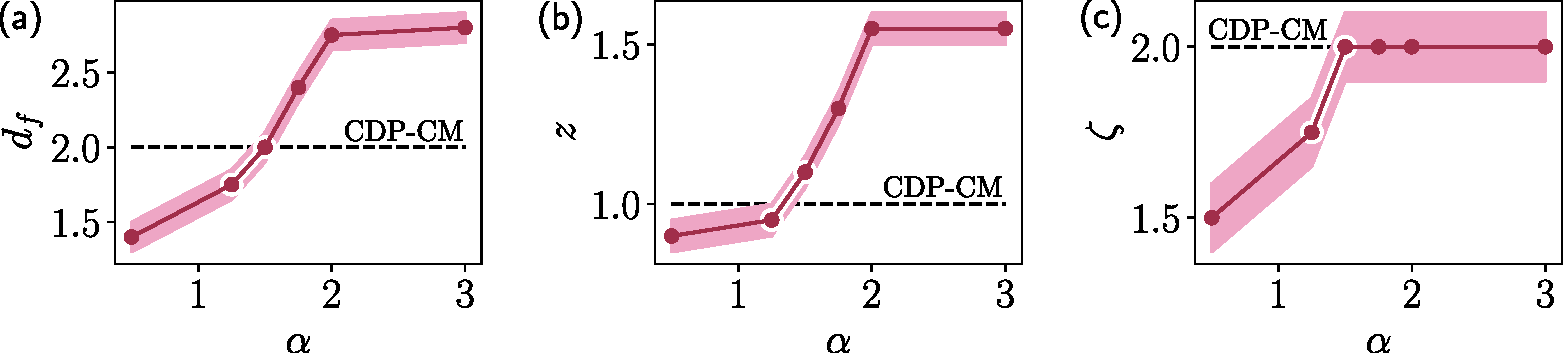
\includegraphics[width=\textwidth]{Chapitre3/Figures/Avalanches/Recap_AvSuspensions.pdf}
	\caption{Évolution des exposants de structure des avalanches $d_f$, $z$ et $\chi$ avec la portée $\alpha$ dans le $\alpha$-ROM en 2D.}
	\label{fig:EvolAvSusp}
\end{figure}

\subparagraph{}Finalement, les propriétés d'avalanche du $\alpha$-ROM suivent une évolution similaire à celle des exposants critiques. Pour $\alpha \gtrsim 1.5$, l'évolution observée est celle obtenue dans le cadre LR-CDP/dépiégeage pour les exposants $\tau$, $\tau^\prime$, $\tau^{\prime\prime}$ et $d_f$ avec des évènements spatialement compacts ($\chi=D$). Pour $\alpha\lesssim 1.5$ cependant, nous observons un comportement hors des bornes du cadre LR-CDP avec des avalanches spatialement fractales.

\section{Conclusion}

\subparagraph{}En conclusion, nous avons caractérisé dans ce chapitre l'influence des interactions médiées sur la transition de réversibilité des suspensions cisaillées cycliquement. Cette caractérisation s'est faite via la définition d'un modèle numérique baptisé $\alpha$-ROM en deux et trois dimensions, contrastant avec le modèle de transport à longue portée LR-ROM établi au chapitre précédent. Celle-ci a alors montré des différences fondamentales entre le comportement critique observé et celui associé au cadre théorique LR-CDP.

\subparagraph{}En déterminant les exposants critiques statiques et dynamiques associés, nous avons mis en évidence l'influence de la portée des interactions sur le comportement critique. Cette influence prenant alors place sur une gamme de portées disjointe de celle observée dans le cadre LR-CDP. De plus, nous avons identifié une gamme de portées sur laquelle la transition se révèle convexe ($\beta >1$) et les fluctuations évanescentes ($\gamma^\prime < 0$), rejoignant alors le modèle de portée infinie ($\alpha=0$) initialement proposé par Mari et al. \cite{mari_absorbing_2022}.

\subparagraph{}Ces observations nous ont poussé à définir un nouveau cadre théorique pour décrire la transition de réversibilité en présence d'interactions médiées. Nous avons alors établi un modèle champ moyen baptisé $\mu$-Hébraud-Lequeux, permettant de rendre compte de la convexité de la transition via la dynamique des particules passives et de comprendre dans une limite champ moyen l'influence de la portée des interactions sur le comportement critique.

\subparagraph{}Enfin, nous avons caractérisé cette famille de transitions par sa dynamique d'avalanche. En réalisant des avalanches à densité de particules fixée, nous avons montré que leur statistique dépend fortement de la portée de l'interaction étudiée. Notamment, les exposants d'avalanche suivent une évolution proche des exposants critiques statiques, délimitant une zone fondamentalement différente du cadre LR-CDP. Dans cette zone de portée où les avalanches dans le cadre LR-CDP sont dans le régime de champ moyen (puisque $\alpha < 3$), les avalanches dans le cadre du modèle $\alpha$-ROM montrent une structure spatialement fractale.